%% 
%% Copyright 2007, 2008, 2009 Elsevier Ltd
%% 
%% This file is part of the 'Elsarticle Bundle'.
%% ---------------------------------------------
%% 
%% It may be distributed under the conditions of the LaTeX Project Public
%% License, either version 1.2 of this license or (at your option) any
%% later version.  The latest version of this license is in
%%    http://www.latex-project.org/lppl.txt
%% and version 1.2 or later is part of all distributions of LaTeX
%% version 1999/12/01 or later.
%% 
%% The list of all files belonging to the 'Elsarticle Bundle' is
%% given in the file `manifest.txt'.
%% 

%% Template article for Elsevier's document class `elsarticle'
%% with numbered style bibliographic references
%% SP 2008/03/01

\documentclass[preprint,12pt]{elsarticle}

%% Use the option review to obtain double line spacing
%% \documentclass[authoryear,preprint,review,12pt]{elsarticle}

%% Use the options 1p,twocolumn; 3p; 3p,twocolumn; 5p; or 5p,twocolumn
%% for a journal layout:
%% \documentclass[final,1p,times]{elsarticle}
%% \documentclass[final,1p,times,twocolumn]{elsarticle}
%% \documentclass[final,3p,times]{elsarticle}
%% \documentclass[final,3p,times,twocolumn]{elsarticle}
%% \documentclass[final,5p,times]{elsarticle}
%% \documentclass[final,5p,times,twocolumn]{elsarticle}

%% For including figures, graphicx.sty has been loaded in
%% elsarticle.cls. If you prefer to use the old commands
%% please give \usepackage{epsfig}

%% The amssymb package provides various useful mathematical symbols
\usepackage{xspace}
\usepackage{amssymb}
\usepackage{amsmath}
\usepackage{subcaption}
\usepackage[printonlyused]{acronym}
%%
\acrodef{AHB}[AHB-PNW]{Advanced Hardwood Biofuels Northwest}
\acrodef{BCAM}{Bioenergy Crop Adoption Model} 
\acrodef{CCSM3}{Community Climate System Model version 3}
\acrodef{CDL}{Cropland Data Layer}
\acrodef{GBSM}{Geospatial Bioenergy Systems Model}
\acrodef{GIS}{Geographical Information System}
\acrodef{IPCC}{Intergovernmental Panel on Climate Change}
\acrodef{mmu}{minimum mapping unit}
\acrodef{NASS}{National Agricultural Statistics Service}
\acrodef{NLCD}{National Land Cover Dataset}
\acrodef{NRCS}{Natural Resources Conservation Service, Department of Agriculture}
\acrodef{NREL}{National Renewable Energy Laboratory}
\acrodef{PNW}{Pacific Northwest}
\acrodef{PRISM}{Parameter-elevation Relationships on Independent Slopes Model} 
\acrodef{SRWC}{short rotation woody crops}
\acrodef{STATSGO}{State Soil Geographic}
\acrodef{USGS}{United States Geological Survey}
\acrodef{SECRETS}{Stand to Ecosystem CaRbon and EvapoTranspiration
Simulator}
%% 3PG acronyms
\acrodef{3pg}[\textsc{3PG}]{Physiological Principles in Predicting Growth}
\acrodef{BLcond}[\ensuremath{BL_{cond}}]{Boundary layer conductance}
\acrodef{dbh}[\ensuremath{dbh}]{Diameter at Breast Height}
\acrodef{DOB}[\ensuremath{DOB}]{Basal Diameter}
\acrodef{LAIt}[\ensuremath{LAI_{T}}]{Target Leaf Area Index}
\acrodef{LAI}[\ensuremath{LAI}]{Leaf Area Index}
\acrodef{NPPdef}[\ensuremath{NPP_{def}}]{$NPP$ deficit}
\acrodef{NPPt}[\ensuremath{NPP_{T}}]{Target Productivity}
\acrodef{NPP}[\ensuremath{NPP}]{Net Primary Productivity}
\acrodef{RP}[\ensuremath{RP}]{Root Productivity}
\acrodef{Rdp}[\ensuremath{R_{\Delta}}]{monthly root contribution}
\acrodef{Re}[\ensuremath{e_{R}}]{root conversion efficiency}
\acrodef{SLA}[\ensuremath{SLA}]{Specific Leaf Area}
\acrodef{WF}[\ensuremath{W_F}]{Foliage biomass}
\acrodef{WS}[\ensuremath{W_S}]{Stem biomass}
\acrodef{WR}[\ensuremath{W_R}]{Root biomass}
\acrodef{W}[\ensuremath{W}]{Plant biomass}
\acrodef{dRres}[\ensuremath{\Delta R_{res}}]{Residual root contribution}
\acrodef{dW}[\ensuremath{\Delta W}]{Total Monthly Growth}
\acrodef{fSW}[\ensuremath{f_\Theta}]{soil water limiter}
\acrodef{fAge}[\ensuremath{f_{age}}]{age growth limiter}
\acrodef{fNutr}[\ensuremath{f_{nutr}}]{nutritional limiter}
\acrodef{fT}[\ensuremath{f_T}]{temperature limiter}
\acrodef{fi}[\ensuremath{f_i}]{Generic growth limiters}
\acrodef{k}[\ensuremath{k}]{radiation extinction coefficient}
\acrodef{lf}[\ensuremath{lf}]{Litter fall}
\acrodef{pRx}[\ensuremath{x_{pR}}]{maximum root fraction}
\acrodef{pR}[\ensuremath{p_R}]{Root allocation}
\acrodef{pfs}[\ensuremath{p_{FS}}]{foliage to stem allocation fraction}
\acrodef{VI}[\ensuremath{VI}]{Volume Index}
\acrodef{sps}[\ensuremath{n_{stems}}]{Stems per stump}
\acrodef{cancover}[\ensuremath{CanCover}]{canopy coverage}
\acrodef{LA}[\ensuremath{LA}]{Leaf Area per stem}
\acrodef{swc}[\ensuremath{\Theta_{c}}]{$f_\Theta$ constant}
\acrodef{swp}[\ensuremath{\Theta_{P}}]{$f_\Theta$ power}
\acrodef{maxAWS}[\ensuremath{S_x}]{Maximum available soil water}
\acrodef{AWS}[\ensuremath{S}]{Available soil water}

% Tests
%\acrodef{HW1}{}
%\acrodef{HW2}{Hardwood Default in Coppice}

%\newcommand{\degree}{\ensuremath{{}^{\circ}}\xspace}
\newcommand{\degree}{\ensuremath{{}^{\circ}}\xspace}

%% The amsthm package provides extended theorem environments
%% \usepackage{amsthm}

%% The lineno packages adds line numbers. Start line numbering with
%% \begin{linenumbers}, end it with \end{linenumbers}. Or switch it on
%% for the whole article with \linenumbers.
%% \usepackage{lineno}
\usepackage{graphicx}
\usepackage{color}
\pdfpagebox5
\usepackage{pgfplots}

\journal{Biomass \& Bioenergy}

\begin{document}

\begin{frontmatter}

%% Title, authors and addresses

%% use the tnoteref command within \title for footnotes;
%% use the tnotetext command for theassociated footnote;
%% use the fnref command within \author or \address for footnotes;
%% use the fntext command for theassociated footnote;
%% use the corref command within \author for corresponding author footnotes;
%% use the cortext command for theassociated footnote;
%% use the ead command for the email address,
%% and the form \ead[url] for the home page:
%% \title{Title\tnoteref{label1}}
%% \tnotetext[label1]{}
%% \author{Name\corref{cor1}\fnref{label2}}
%% \ead{email address}
%% \ead[url]{home page}
%% \fntext[label2]{}
%% \cortext[cor1]{}
%% \address{Address\fnref{label3}}
%% \fntext[label3]{}

\title{Modeling Poplar Growth as a Short Rotation Woody Crop for Biofuels in the Pacific Northwest}

%% use optional labels to link authors explicitly to addresses:
%% \author[label1,label2]{}
%% \address[label1]{}
%% \address[label2]{}

\author[lawr]{Q. J. Hart}
%\author[en]{N. C. Parker}
%\author[plant]{B.L. Yeo}
%\author[en]{V. Bandaru}
%\author[lawr]{J. R. Merz}
\author[pfc]{A. Cooke}
\author[bioag]{B. M. Jenkins}

\address{Department of Land, Air, and Water, University of California, Davis, USA\fnref{lawr}}
\address{Precision Forestry Cooperative, University of Washington, USA\fnref{pfc}}
%\address{Department of Plant Sciences, University of California, Davis, USA\fnref{plant}}
%\address{Energy Institute, University of California, Davis, USA\fnref{en}}
\address{Department of Biological and Agricultural Engineering, University of California, Davis, USA\fnref{bioag}}

\begin{abstract}
  Predicting the economic viability and environmental sustainability
  of a biofuels industry based on this feedstock requires spatial
  predictions of the growth and yield of \acf{SRWC} under various
  environmental conditions and throughout large regions.  The \acf{3pg}
  model was modified for modeling SRWC, particularly for poplar
  plantation methodologies.  This included developing a sub-model
  which takes into account the coppicing strategy for harvesting
  poplar that allows a monthly growth contribution from an existing
  root mass.

  The parameterized model was then applied to the entire Pacific
  Northwest of the United States, using appropriate climatological and
  soil input data.  Existing agricultural patterns were used to
  estimate regional water availability for irrigation, and for
  nonirrigated regions, land cover features including ownership,
  slope , soil salinity and water table depth where used to limit
  predictions to areas with a real potential to support a \ac{SRWC}
  plantation.

  Results can be integrated with other models that allow for
  optimizing the crop selection and biorefinery site selection.
  Important findings from the model include; validation of the
  \ac{3pg} model for coppiced \ac{SRWC} plantings, estimates of
  biomass feedstock yields under different irrigation patterns and
  weather conditions, and annual estimates for feedstock availability
  when combined with crop adoption scenarios.

\end{abstract}

\begin{keyword}
%% keywords here, in the form: keyword \sep keyword
  Short rotation woody crops \sep Poplar \sep \ac{3pg} \sep Yield
  estimations \sep Pacific Northwest, USA.

%% PACS codes here, in the form: \PACS code \sep code

%% MSC codes here, in the form: \MSC code \sep code
%% or \MSC[2008] code \sep code 

\end{keyword}

\end{frontmatter}

%% \linenumbers

%% main text
\section{Introduction}
\label{sec:introduction}
%% Text of abstract
The \acf{AHB} is a consortium of university and industry partners
investigating the development of a sustainable hardwood biofuels
industry in Washington, Oregon, Northern California and Western Idaho
in the U.S.  Inspired in part by the U.S. Energy Independence and
Security Act 2022 targets for renewable fuel, \ac{AHB} is carrying out
research and development to support a system for growing and
converting hardwoods, such as hybrid poplars, into liquid biofuels
that are fully compatible with existing infrastructure.

To support economic and environmental models for a biofuels industry,
spatial predictions of the growth and yield of \acf{SRWC} under
various environmental conditions and throughout the entire \acf{PNW},
the \acf{3pg} model was utilized.  The model was modified for
\ac{SRWC}, particularly for poplar plantation methodologies.

A physiological growth model such as \ac{3pg} is advantageous because
it allows variation of growth parameters and assumptions regarding
management practices for poplar species.  In addition to biomass growth
and yield estimations, because it is a canopy carbon balance model,
allocations for both above and below ground biomass can be tracked for
life-cycle analysis of the product fuels.

The original \ac{3pg} model does not include coppicing as a management
practice, which is problematic as it cannot reasonably account for
post-coppicing regrowth.  The extended model includes coppicing with a
general model that allows a monthly growth contribution from an
existing root mass.  The model specifies a relatively small
contribution of aboveground growth from the accumulated root mass
after coppicing in order to initiate the next cycle of production.

The \ac{3pg} model was validated against a number of field studies
related to the growth of poplar as a \ac{SRWC} biofuel feedstock.  The
parameterized model was then applied to the entire Pacific Northwest
region, using appropriate climatology and soil input data.  Climate
data included both historical patterns as well as predicted patterns
from simulations predicting climate change.  These inputs produce
poplar yield prediction maps and expected bounds on the variation of
these yields useful for determining when it becomes economically
feasible for poplar to be grown within the study area. 

This yield model is overlaid with surface and land cover
parameters to predict yields for potential plantation locations.
Yield maps are the results of running the \ac{3pg} model for the
entire \ac{AHB} region. 

With appropriate input information, the \ac{3pg} model can predict
yields for the entire Pacific Northwest study region, under various
irrigation scenarios.  When linked with models of crop adoption,
annual feedstock estimates are possible.

\section{Methods and Calculation}

The main goal of this study was to create spatially explicit poplar
growth potential for the \ac{PNW} that can inform our participants and
subsequent modeling efforts on the predicted yields from \ac{SRWC}
plantations.

The study area, the Pacific Northwest of the United States,
incorporates Washington, Oregon, Northern California, and Western
Idaho.  This definition of the \acs{PNW} is somewhat inclusive in the
South, including the northern part of California~(Figure~\ref{fig:grid}).

A regular grid partitions the region.  The individual pixel size is
relatively coarse $8192 \times 8192$ (m\^2), and designed to reduce
some of the complexity of subsequent regional optimization models.
The projection is an Albers equal area projection with standard
longitude 120\degree West, and parallels at latitudes 41\degree and
47\degree North~\cite{Butler}. This projection insures the pixels
maintain a constant area, while maintaining good conformity for
transportation networks.  The pixel edge length, $8192 = 2^{13}$~(m)
is defined as a binary factor to allow easy scaling up and down of the
data to different resolutions while maintaining common edges.  For
example, the \ac{NLCD} dataset, used in this study, was originally
imported and projected to $2^5$ (m), and aggregated upwards to
determine percentages of each landcover type for each
pixel~(Figure~\ref{fig:land}).

\begin{figure}[hp]
  \centering
  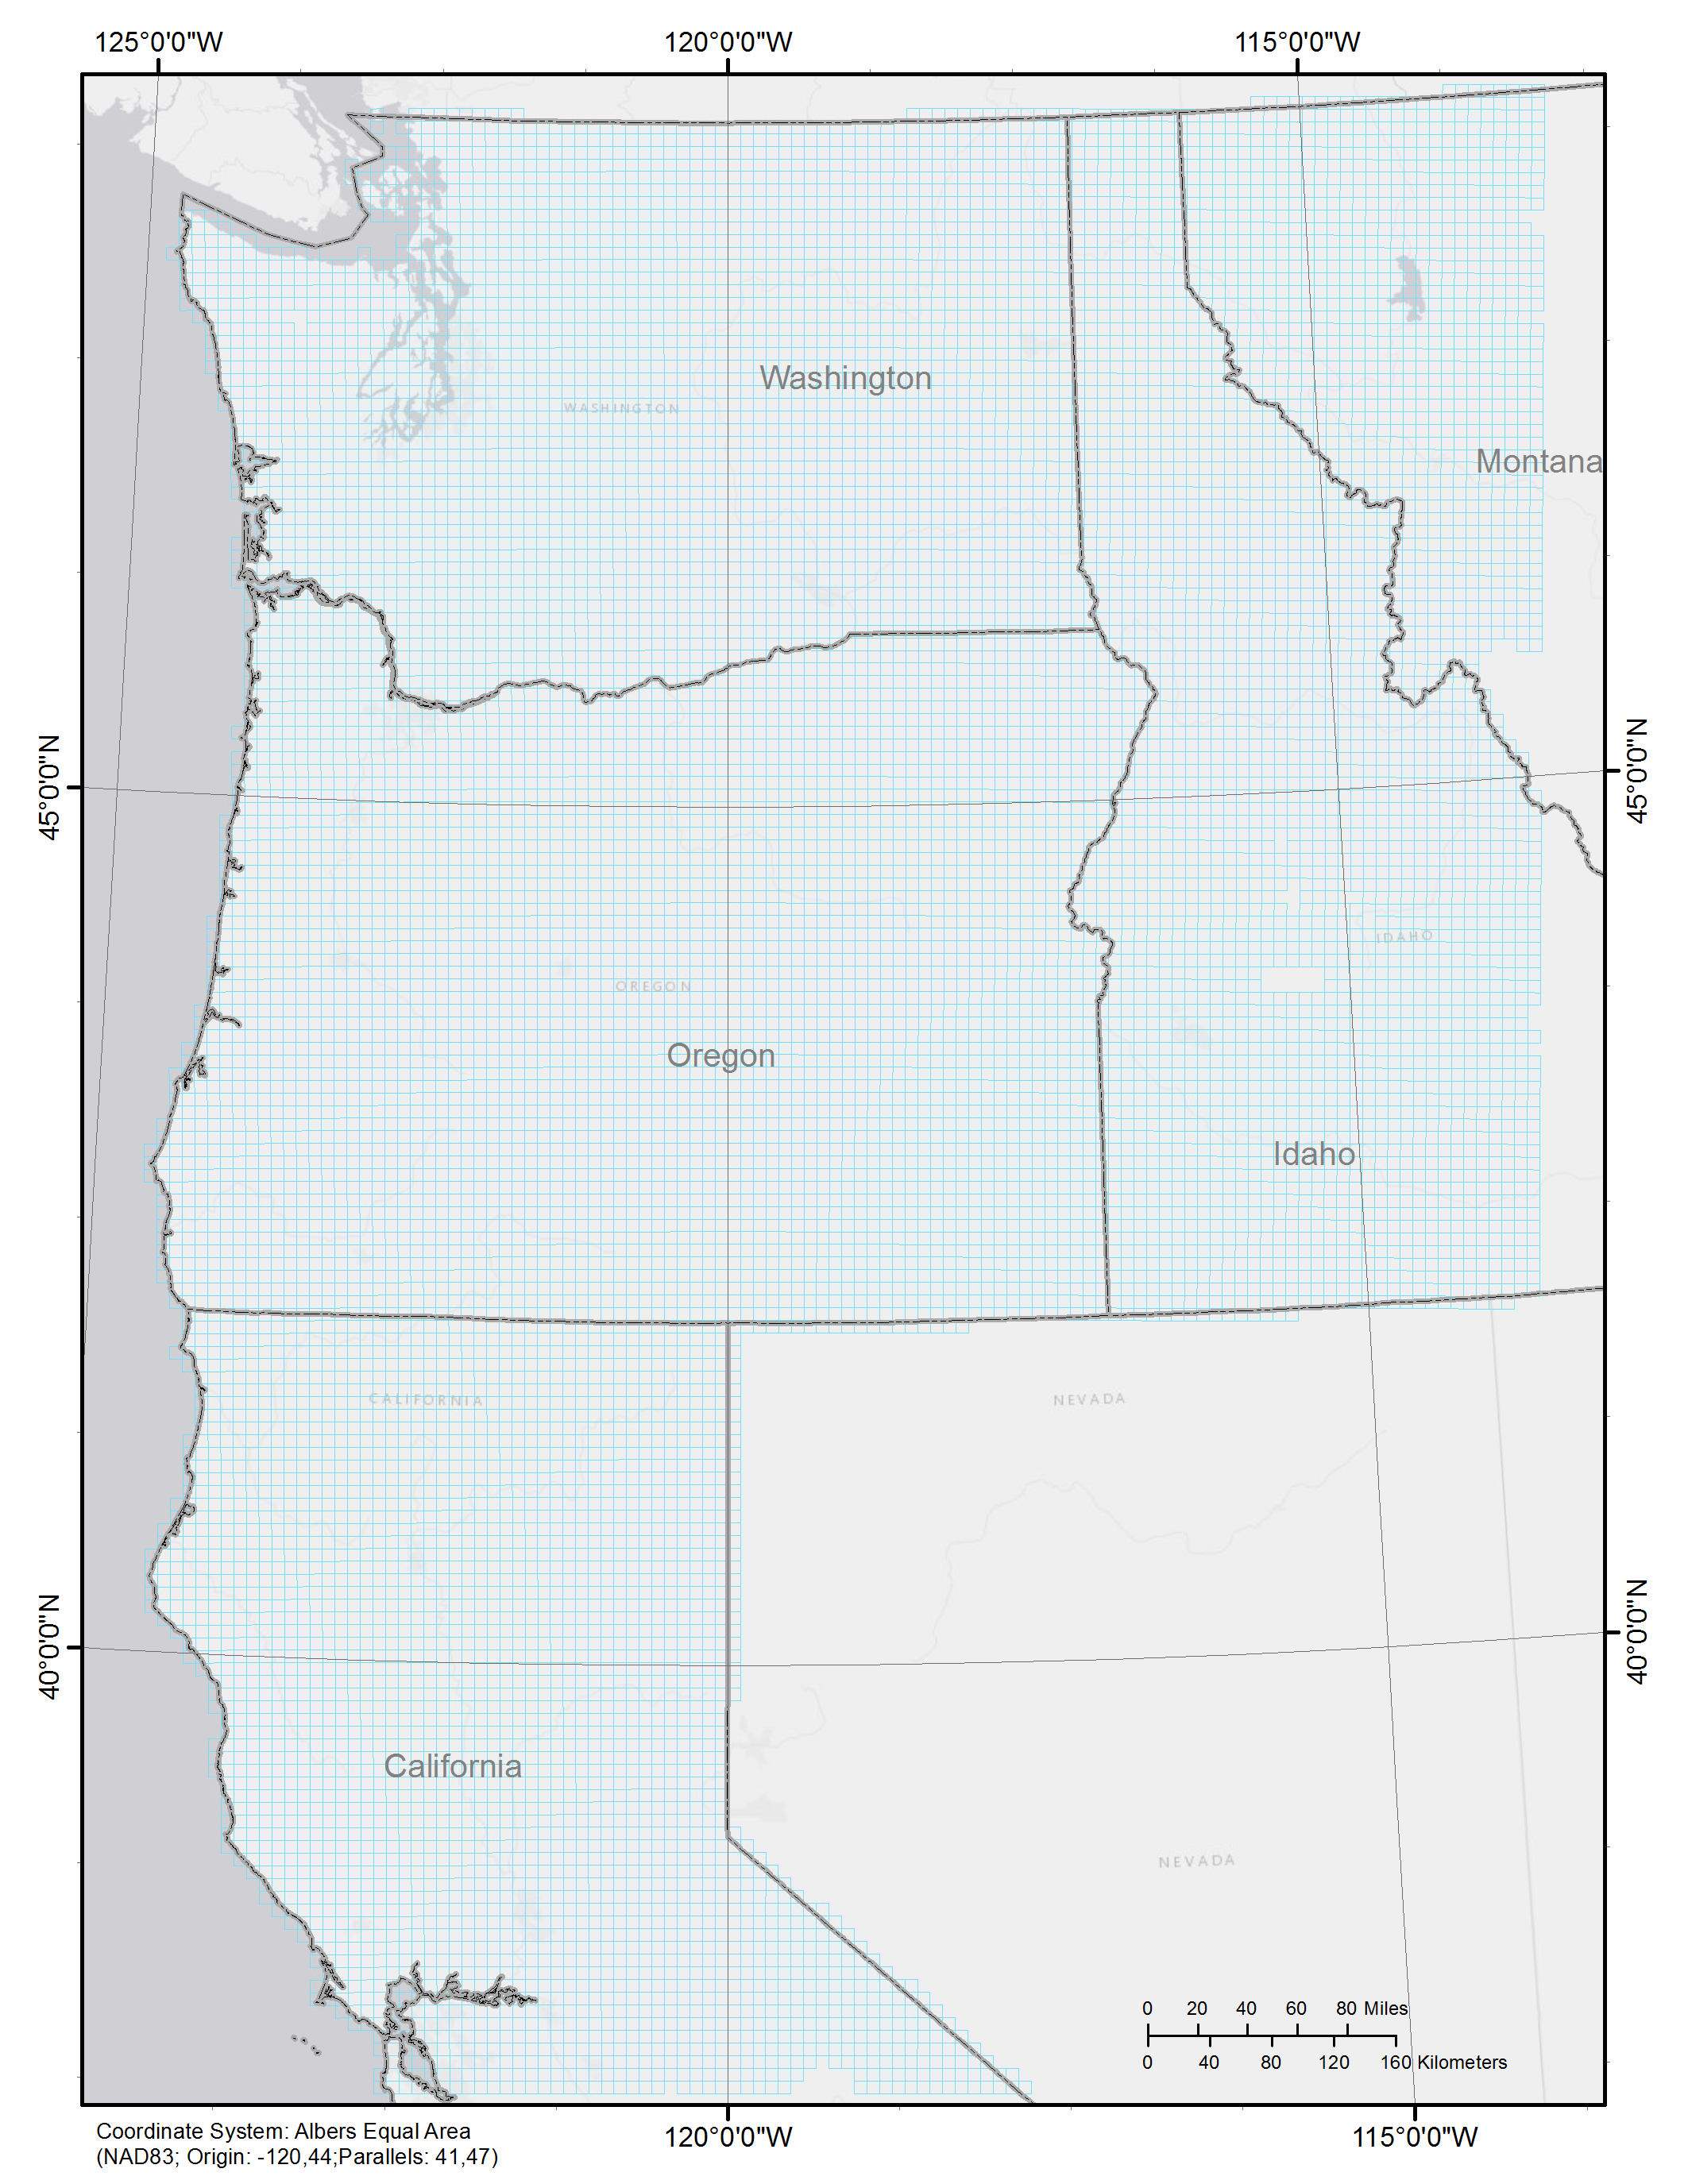
\includegraphics[width=1.0\linewidth]{grid}
  \caption{Location of the study area, with grid layer overlaid.}
  \label{fig:grid}
\end{figure}

Data processing was carried out within a postgresql database, with the
postgis geospatial extensions~\cite{pgsql,Holl2009,postgis}.
Specialized calculations were implemented as postgresql functions, using
various scripting languages; SQL, PLSQL, Javascript, and R.

% \begin{table}
%   \centering
%   \begin{tabular}[hp]{|l|l|}
%     \hline
%     Parameter & Source(s) \\
%     \hline
%     Temperature & \acs{PRISM} \\
%     Precipitation & \acs{PRISM} \\
%     Solar Radiation & \ac{USGS} \\
%     \hline
%   \end{tabular}
%   \caption{Required Model Inputs}
%   \label{tab:input}
% \end{table}

\subsection{\acs{3pg} Model Formulation}
\label{sec:3pg}

The \acf{3pg} model~\cite{Landsberg1997, landsberg2010physiological,
  Sands2004} is the primary tool used for the \ac{SRWC} yield
estimations, and takes as inputs weather data, soil parameters, site
factors, including soil parameters, initial stocking conditions,
management practices, and species
definitions~(Figure~\ref{fig:overview}).  The \ac{3pg} model is run at
a monthly timestep. At each step the physiological parameters are
calculated and carried forward to the next month.  These incremental
physiological parameters can be compared to model predictions with
field results at multiple stages in the plantation's history.

\begin{figure}[p]
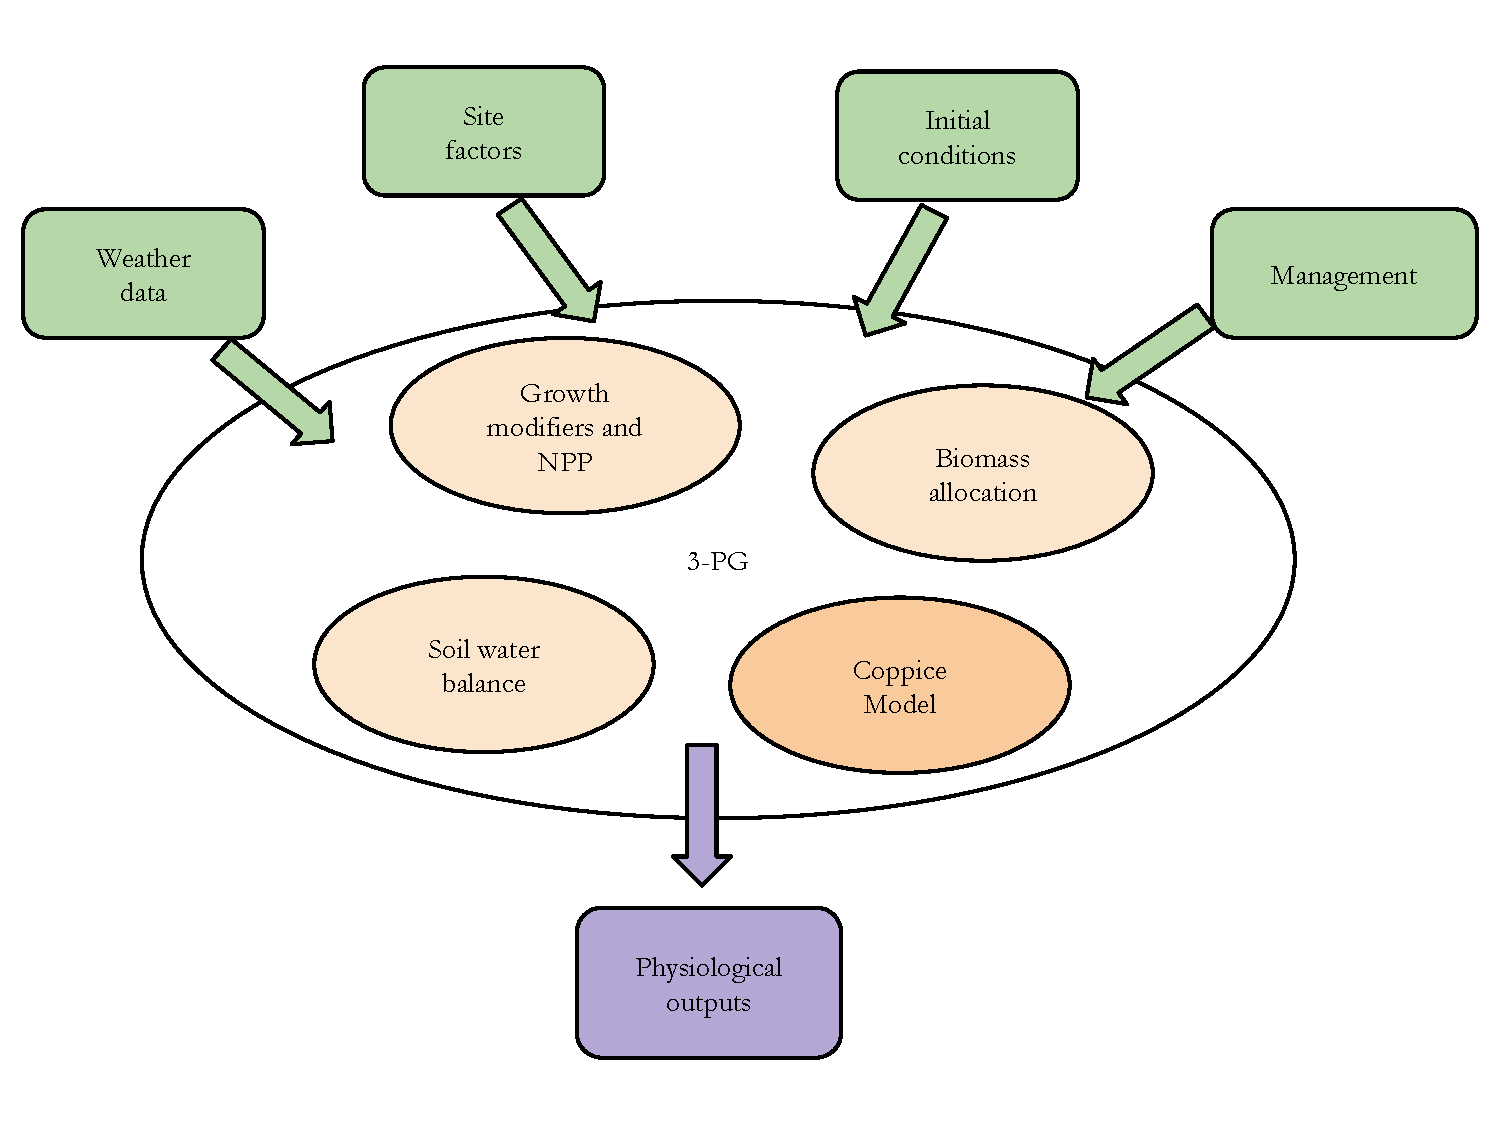
\includegraphics[width=\linewidth]{model_overview}
\caption{ The \ac{3pg} model's main inputs.  Running at a monthly timestep, with
appropriate input parameters, the model predicts tree growth and a
number of other parameters.}
\label{fig:overview}
\end{figure}

The original \ac{3pg} model allocates production from transpiration
into the creation of new roots, stems and foliage.  After coppicing
however, the model has no mechanism to increase start of re-growth
from the root.  A simple coppicing model has been developed to add an
additional production from the root system after
coppicing~\cite{Hart2014}.  When a \ac{SRWC} is coppiced, there is a
surfeit of root mass when compared to the aboveground biomass.  This
surfeit is allowed to contribute some of this surfeit as an additional
production at each monthly timestep, along with the \ac{NPP} of the
original model.  The seasonal timing of any root contribution is
moderated by comparing the actual \ac{NPP} to a potential \ac{NPP} the
tree would have a specified target \ac{LAI}.  This difference serves
as a maximum limit for the root contribution.  Using a potential
\ac{NPP} from a target \ac{LAI} serves two purposes. First, it allows
root contributions up to, but not beyond a certain foliage amount, as
specified by the \ac{LAI}.  More importantly, since the root
contribution is tied to a potential \ac{NPP}, the method times
regrowth with climatic conditions that are favorable for growth, and
does not initiate growth when conditions are not favorable.  A maximum
allowable monthly root contribution fraction limits the total
contribution for any one month, and affects the length of time for
the contribution to be made.  In poplar plantations, where plantings
are initiated with bare cuttings as propagation, the initial growth
is modeled the same way, however with different parameters to model
initial root dynamics.

Hart et al.~\cite{Hart2014} validated a set of \ac{3pg} tree
parameters, primarily following a poplar parameterization of Headlee
et al.~\cite{Headlee2012} that reasonably model a generic poplar
species.  In addition, and set of 6 additional variations on these
parameters were derived to match reported field study results.  These
sets of parameters were used as an ensemble of inputs to the yield
predictions below.

\subsubsection{Climatic and Radiation Data}
\label{sec:climate}

%http://cses.washington.edu/cig/pnwc/pnwc.shtml
%http://en.wikipedia.org/wiki/Climate_of_California

The Pacific Northwest weather patterns are influenced primarily by the
Pacific storm track, which brings in the bulk of precipitation in the
months of October through March, and the location and size of the
mountain ranges, which moderate both the precipitation, and the
temperatures throughout the year.

In order to predict temperatures and precipitation on the near term,
the \acf{PRISM} dataset was used~\cite{Daly2008a}.  \ac{PRISM}
extrapolates station data spatially to a uniform grid using weights
derived from the physiographic similarity of the station to the grid
cell. These similarity measures include location, elevation, coastal
proximity, topographic facet orientation, vertical atmospheric layer,
topographic position, and orographic effectiveness of the terrain.
\ac{PRISM} data is available on a 2.5 minute geographic grid.

16 years of \ac{PRISM} data were interpolated (cubic spline) to the
\ac{AHB} grid averaged to determine a representative weather pattern
used near term modeling for the \ac{AHB} yield predictions.
Figure~\ref{fig:temp} shows annual mean temperature and total
precipitation variation of the region.  Isolines show the standard
deviation between annual mean temperature to the monthly mean
temperature.  Similarly isolines shown on the precipitation map show
the maximum monthly contribution of preciptation.

\begin{figure}[hp]
  \centering  
  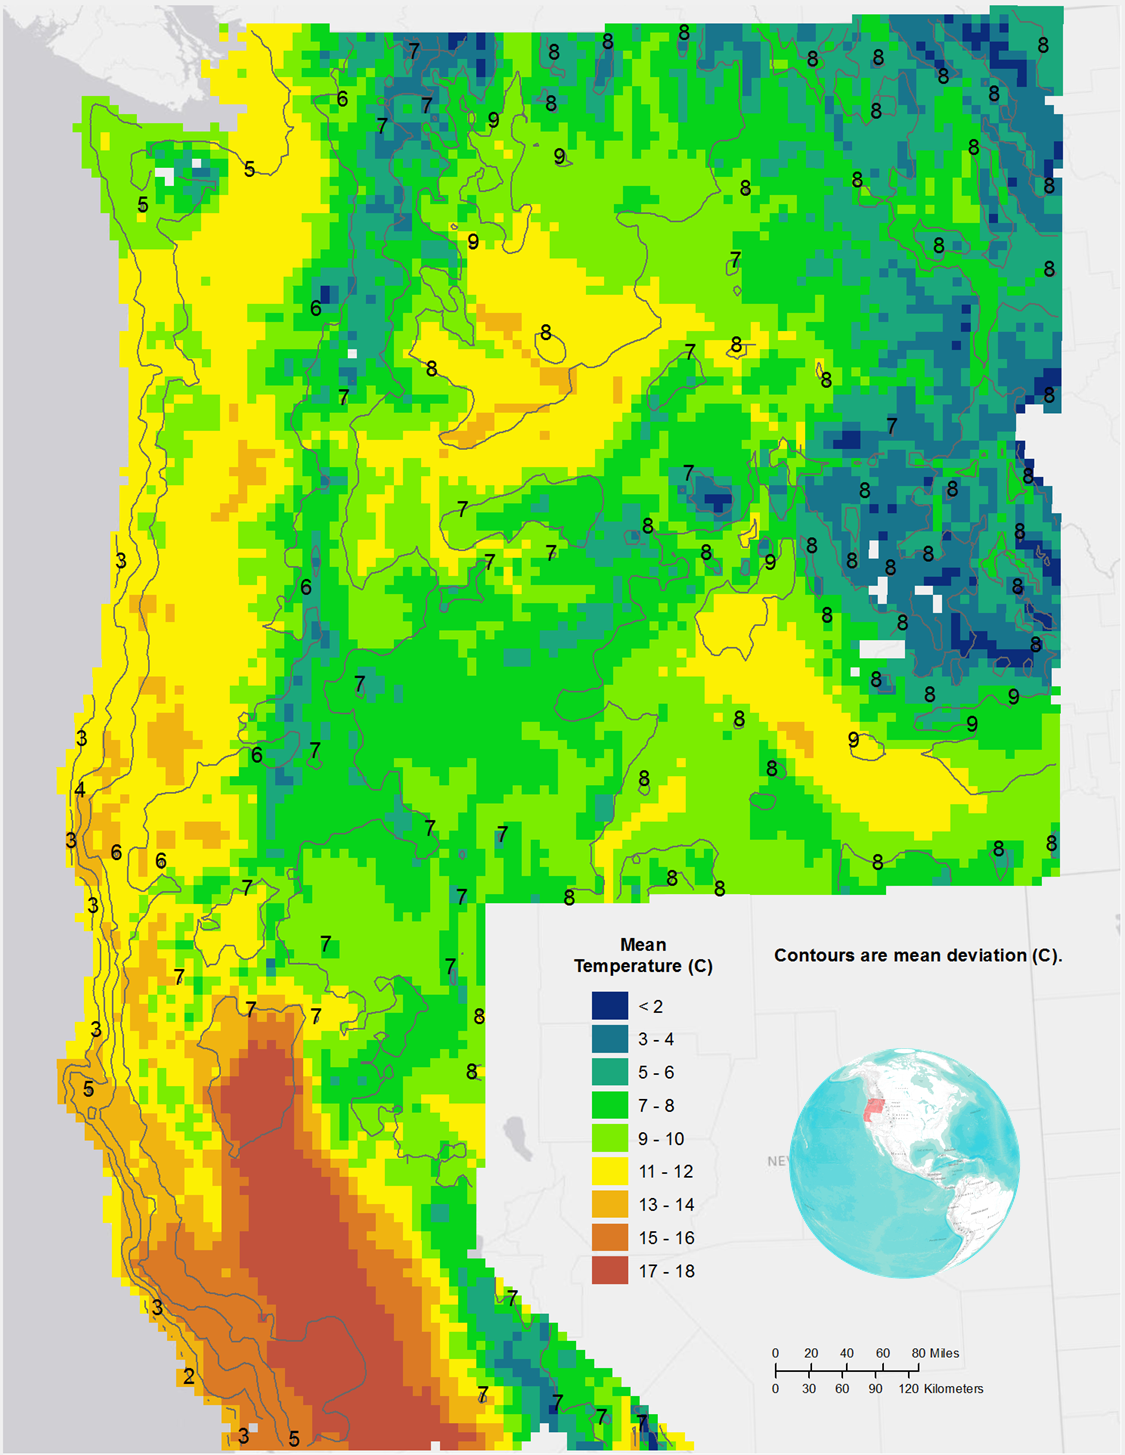
\includegraphics[width=1\linewidth]{temp}  
\caption{Mean annual Temperature, with isolines showing the standard deviation in monthly temperature.}
  \label{fig:temp}
\end{figure}

\begin{figure}[hp]
  \centering  
  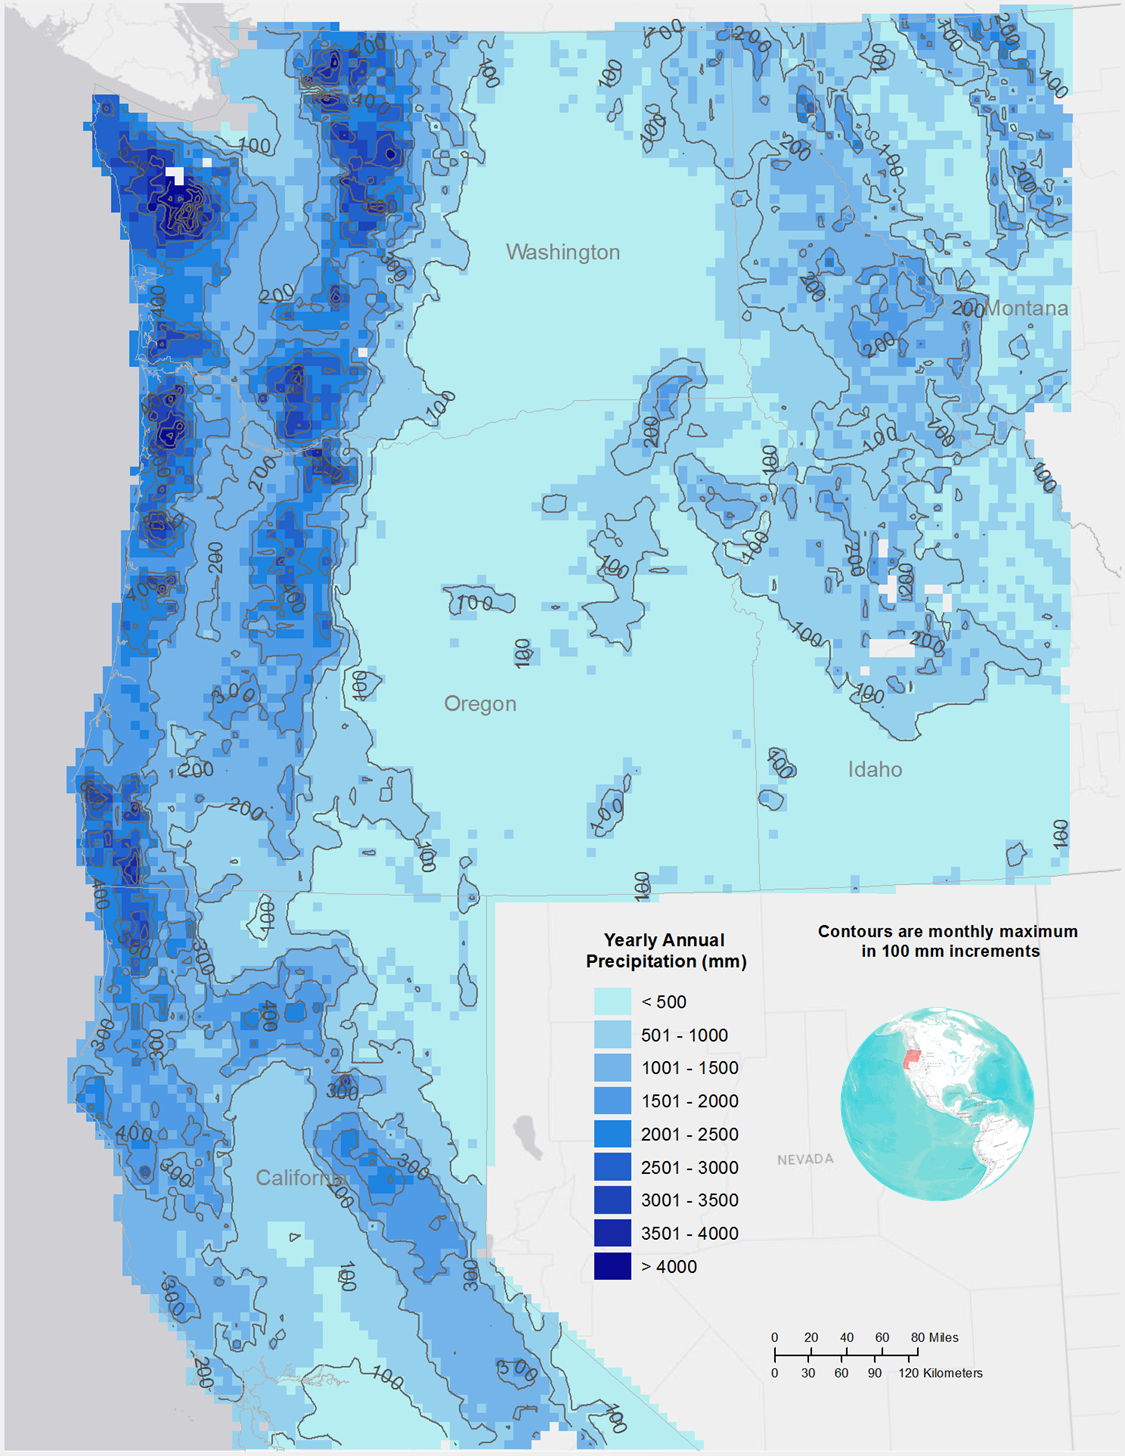
\includegraphics[width=1.0\linewidth]{precip}  
\caption{Total annual rainfall, with iso lines showing the maximum monthly rainfall.}
  \label{fig:precip}
\end{figure}

In order to determine incoming monthly solar radiation, monthly
\acf{NREL} global incident radiation data were
utilized~\cite{perez2002new}.  The incident radiation data product
provides monthly average and annual average daily total solar resource
averaged over surface cells of 0.1 degrees.  Hourly radiance images
from geostationary weather satellites, daily snow cover data, and
monthly averages of atmospheric water vapor, trace gases, aerosols are
used to calculate the hourly total direct and diffuse insolation
falling on a horizontal surface.  Existing ground measurement stations
validate the data where available.

The incident radiation data is available on a gridded format with a
scale similar to this project and is interpolated (cubic-spline)
onto the \ac{AHB} grid for use.

\subsubsection{Soil Parameters}
\label{sec:soil}

\ac{3pg} uses a single layer soil model that maintains an estimate of
the amount of water available at any timestep in the model.  In
addition, \ac{3pg} includes a growth limiter related to the available
water in the soil, and the soil type.  These require a number of soil
parameters.

These parameters are all determined using the \acf{STATSGO}
database~\cite{SoilSurveyStaff2012-STATSGO}.  \ac{STATSGO} is a
national soil database, distributed by the \ac{NRCS}.  \ac{STATSGO}
maps are designed for regional studies, and the soil inventories are
typically generalized from more detailed surveys, or from a
combination of ancillary datasets.  Individual \ac{STATSGO} areas can
contain multiple soil components, and the map units are linked to
attributes the soil data base which gives the proportionate extent of
the component soils and their associated properties.  The \ac{mmu} is
about 625 (ha).  For each pixel in the modeling grid, intersecting map
units are averaged for the estimated pixel values.  1887 different
soil were used, contributing anywhere from 144 to 1.3M (ha).

\ac{maxAWS} defines the maximum holding capacity of the soil.
\ac{maxAWS} is directly taken from the \ac{STATSGO} database which
determines the maximum water holding capacity through the complete
horizon over the topmost 1 (m) of soil (Figure~\ref{fig:aws}).

\begin{figure}
  \centering
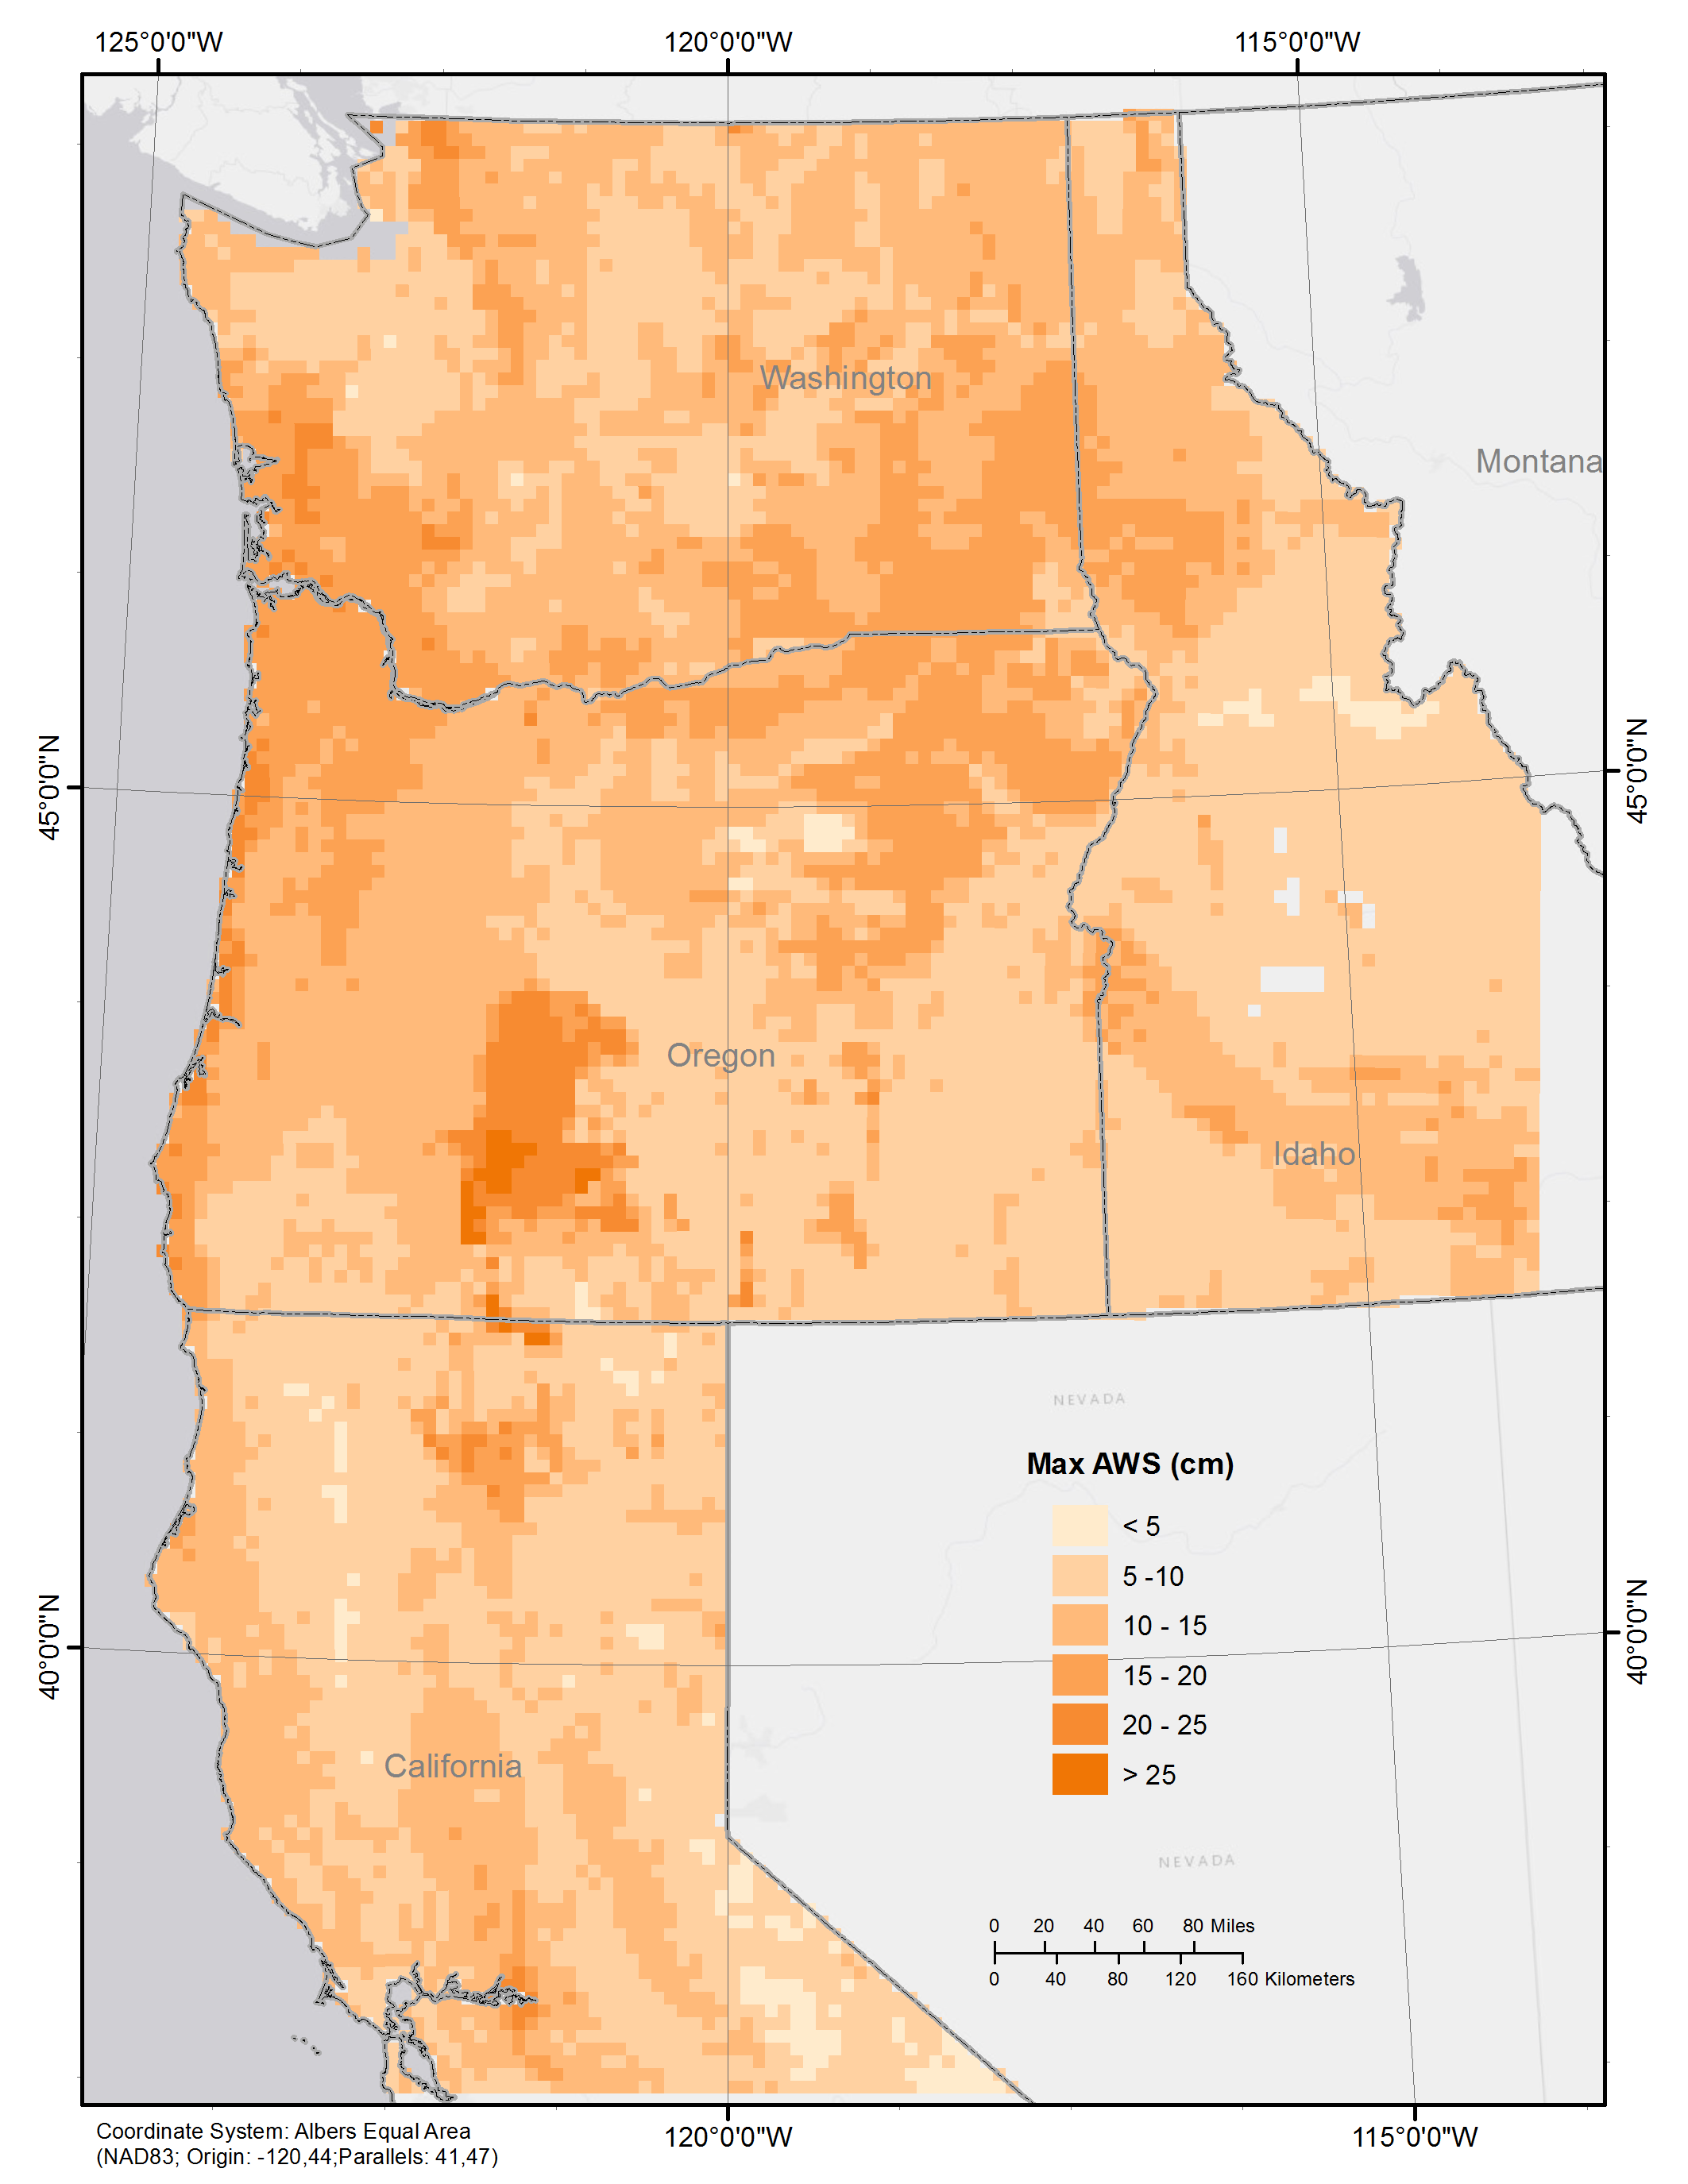
\includegraphics{maxaws}
  \caption{\ac{STATSGO} derived maximum available water estimates. }
  \label{fig:aws}
\end{figure}

The limiter \ac{fSW} is parameterized with two values, \ac{swp} and
\ac{swc} are functions of the soil type (Figure~\ref{fig:soil}.  The
soil type is determined from \ac{STATSGO} report  percentages of
silt sand and clay within each soil component.

%\begin{equation*}
%\acs{fSW} = \frac{1-(1-\acs{AWS}/\acs{maxAWS})^{\acs{swp}}}{1+((1-\acs{AWS}/\acs{maxAWS})/\acs{swc})^{\acs{swp}}}
%\end{equation*} 

\begin{figure}
  \centering
  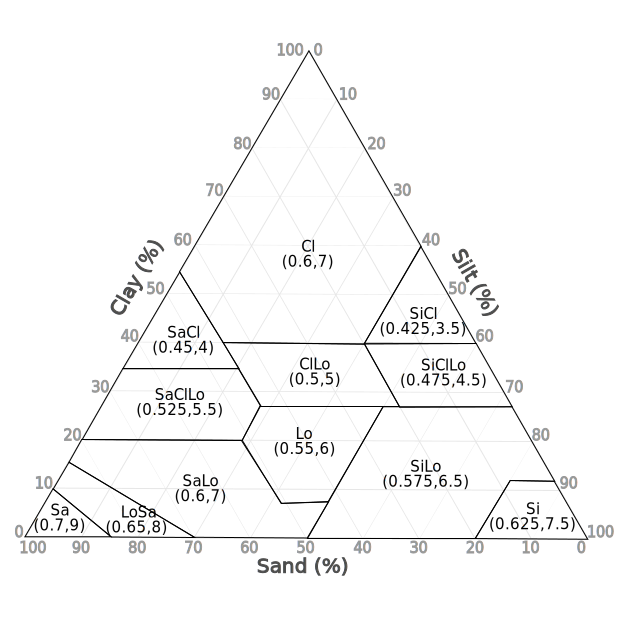
\includegraphics[width=0.45\linewidth]{soil_triangle}
    \begin{tikzpicture}
    \begin{axis}[
      name=fsw,
      xmin=0,xmax=1,
      xtick={0,.2,.4,.6,.8,1},
      xticklabels={0,.2,.4,.6,.8,1},
      xlabel=$\acs{AWS}/\acs{maxAWS}$,
      ymin=0,ymax=1,
      ytick={0,.2,.4,.6,.8,1},
      yticklabels={0,.2,.4,.6,.8,1},
      ylabel=$\acs{fSW}$,
      no markers,
      width=0.45\linewidth,
      height=0.45\linewidth,
      every axis plot/.append style={line width=1pt},
      legend entries={sand,clay,silt},
      legend style={
        at={(0.5,1.0)},anchor=south,legend columns=-1,yshift=2pt}
      ]
      \addplot+[color=red] table [x=awsp, y=Sand, col sep=comma] {soil-fsw.csv};
      \addplot+[color=orange] table [x=awsp, y=Clay, col sep=comma] {soil-fsw.csv};
      \addplot+[color=green] table [x=awsp, y=Silt, col sep=comma] {soil-fsw.csv};
    \end{axis}
  \end{tikzpicture}

  \caption{\acs{swc} and \acs{swp} as determined by soil composition.  Included is a graph for the function $\acs{fSW} = \frac{1-(1-\acs{AWS}/\acs{maxAWS})^{\acs{swp}}}{1+((1-\acs{AWS}/\acs{maxAWS})/\acs{swc})^{\acs{swp}}}$ for sand,silt and clay. }
  \label{fig:soil-triangle}
\end{figure}

\subsection{Land Classification and Irrigation}
\label{sec:land}

Available climatic data makes it possible to make estimations for
poplar growth throughout the \ac{PNW} region.  This may provide
interesting comparisons of changes in yield, but is not very suitable
for determining regional trends, as not all lands are equally likely
to be available for poplar plantations.  Variables like land
ownership, topography and salinity, influence the technical capability
of growing poplar.  

In addition, the ability to irrigate a poplar plantation can have
large effects on the predicted yields of poplar.  Determining which
areas in the \ac{PNW} region are liable to be available for irrigation
can significantly influence regional polar harvest estimations.  

In order to limit the areas within the \ac{AHB} region to areas that
are technically suitable to poplar plantations, a set of masks were
used, derived from a suitability analysis for potential plantation
locations~\cite{Cooke2014}. Permanently non-suitable land was
identified for removal from consideration. Lands under Federal
ownership~\cite{NationalAtlasoftheUnitedStates201} and currently
developed land~\cite{nlcd2011} were excluded from consideration.
Physical features including slopes greater than 15\%~\cite{Gesch2007},
and soil salinity greater than 4 (dS / m) were also
excluded~(Figure~\ref{fig:nonirrigated_yield}).

The land suitability study included other factors for poplar
suitability; nine variables considered important for poplar growth
were identified: growing season precipitation, temperature, and
length; soil texture and drainage, pH, salinity, and depth; water
table depth; and slope.  Most of these parameters are included more
explicitly in the \ac{3pg} model, and directly affect yield
predictions.  Soil salinity and pH have not yet been integrated into
the \ac{pg} model.

% References FAO. 1976. FAO A framework for land evaluation. Soils Bulletin 32. Food and Agriculture Organization of the United Nations, Rome (1976).

Available water for irrigation is a difficult question when dealing
with crops in the \ac{PNW}.  Irrigation is a combination of
availability and rights, that is had to track on a regional scale.
However, one aspect of irrigation is that if it's available it is
likely being used currently.  Therefore, for determining irrigated
yield predictions for poplar, a mask of existing irrigated
agricultural areas was used.  These locations were determined in two
steps.  First, the a cropland data layer was used to spatially locate
agricultural crops in the region.  The USDA, NASS Cropland Data Layer
(CDL) is a nationally available raster of crop specific land cover
data layer with a ground resolution of 30 meters.  The CDL is produced
using satellite imagery with a classification emphasis on agricultural
land cover~\cite{cdl2011}.  The CDL was projected unto the \ac{AHB}
region as a scale of $2^5$.  Individual pixels from the CDL were then
aggregated within the larger model's $2^13$ size pixels to determine
fractional composition of each large pixel~(Figure~\ref{fig:land}.  An
additional step was used to adjust the total area in each county to
the values of hectares reported to the \ac{NASS}.  \ac{NASS} publishes
U.S., State and County agricultural statistics for many
commodities~\cite{nass-quick-stats}.  Later modeling efforts rely on
the \ac{NASS} reported hectares of the various commodities harvested.
This was accomplished by uniformly adjusting the CDL derived pixel
fractions, (the \ac{AHB} 8192 edge length pixels) so that sum of pixel
fractions over nay county in the ac{AHB} region match the reported
number of hectares harvested for that county and commodity.  This
method allows the spatial patterns of the CDL to be retained with
fractions that add to the \ac{NASS} reported values.

\begin{figure}[hp]
  \centering
  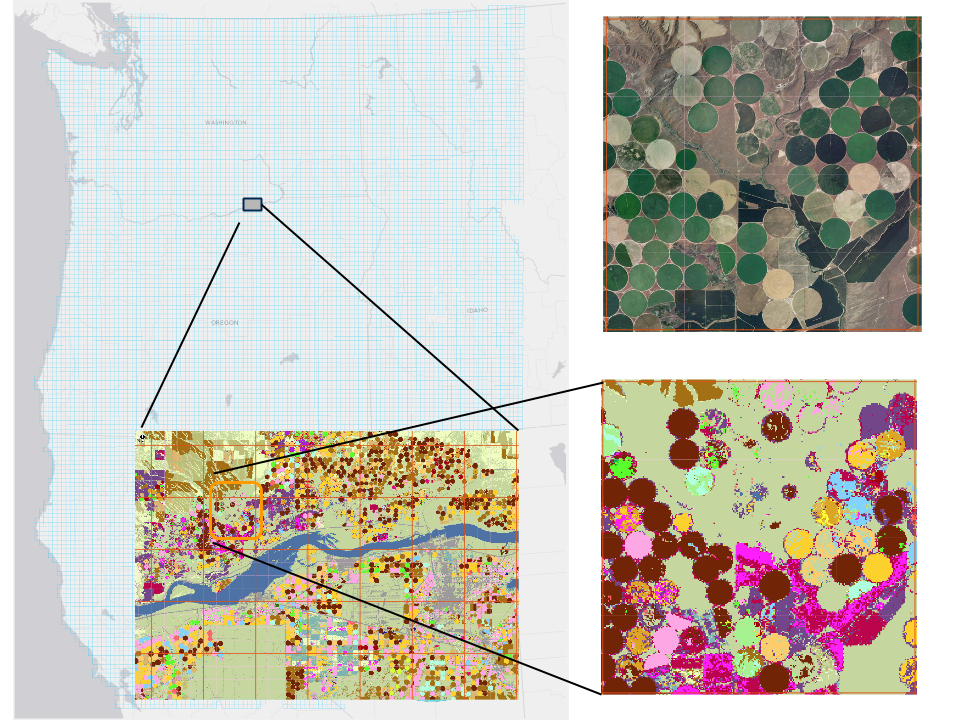
\includegraphics[width=1\linewidth]{land.png}
  \caption{Agricultural Land Classification.  Each \ac{AHB} pixel is made up of
    many remotely sensed derived \ac{CDL} crop classifications.  This
    are aggregated to determine fractional amount of coverage for each
    \ac{AHB} pixel. }
  \label{fig:land}
\end{figure}

\subsection{Climate Change}
\label{sec:climate}

To demonstrate the effect of potential climate change on yield
predictions in the near future, the A1B climate change scenario was
used as an example for predicting yields with a plantation initially
planted in 2040.

The A1B scenario predicts a balanced utilization of available energy
sources, with similar improvement rates applied to all energy supply
and end-use.  The future is one of rapid economic growth, global
population that peaks in mid-century and declines thereafter, and a
rapid introduction of new and more efficient
technologies~\cite{IPCC2007,Parry2007}.

Estimations of the expected change in temperature and precipitation
were derived from the \ac{CCSM3}.  The \ac{CCSM3} is a climate model
with components including the atmosphere, ocean, sea ice, and land
surface. \ac{CCSM3} is designed to produce realistic simulations over
a wide range of spatial and spatial resolutions.  The coarse
\ac{CCSM3} predictions are available at 0.5 degree grid cells.
Estimations of change in the next fifty years were used in these
climate change estimations.

The \ac{CCSM3} estimations cannot be used directly, especially
comparatively to the current estimations using the \ac{PRISM} data.
This is because when comparing the \ac{CCSM3}'s somewhat coarse scale
estimations, to the more detailed \ac{PRISM} estimations the current
(2000-2014) predictions exhibit bias.  Therefore, the \ac{CCSM3}
estimations were used to determine the predicted change in temperature
and precipitation for the \ac {AHB} region, and these changes were
then applied to the current \ac{PRISM} estimations. For example, the
40 year change in temperature, and precipitation for the A1B scenario
shows a mean increase in temperature of about 1\degree Celsius, with
larger changes in the south and west.  Mean annual precipitation
decreases by about 100 (mm) throughout the region with larger changes
in along the coast~(Figure~\ref{fig:change}).

\begin{figure}[hp]
  \centering
  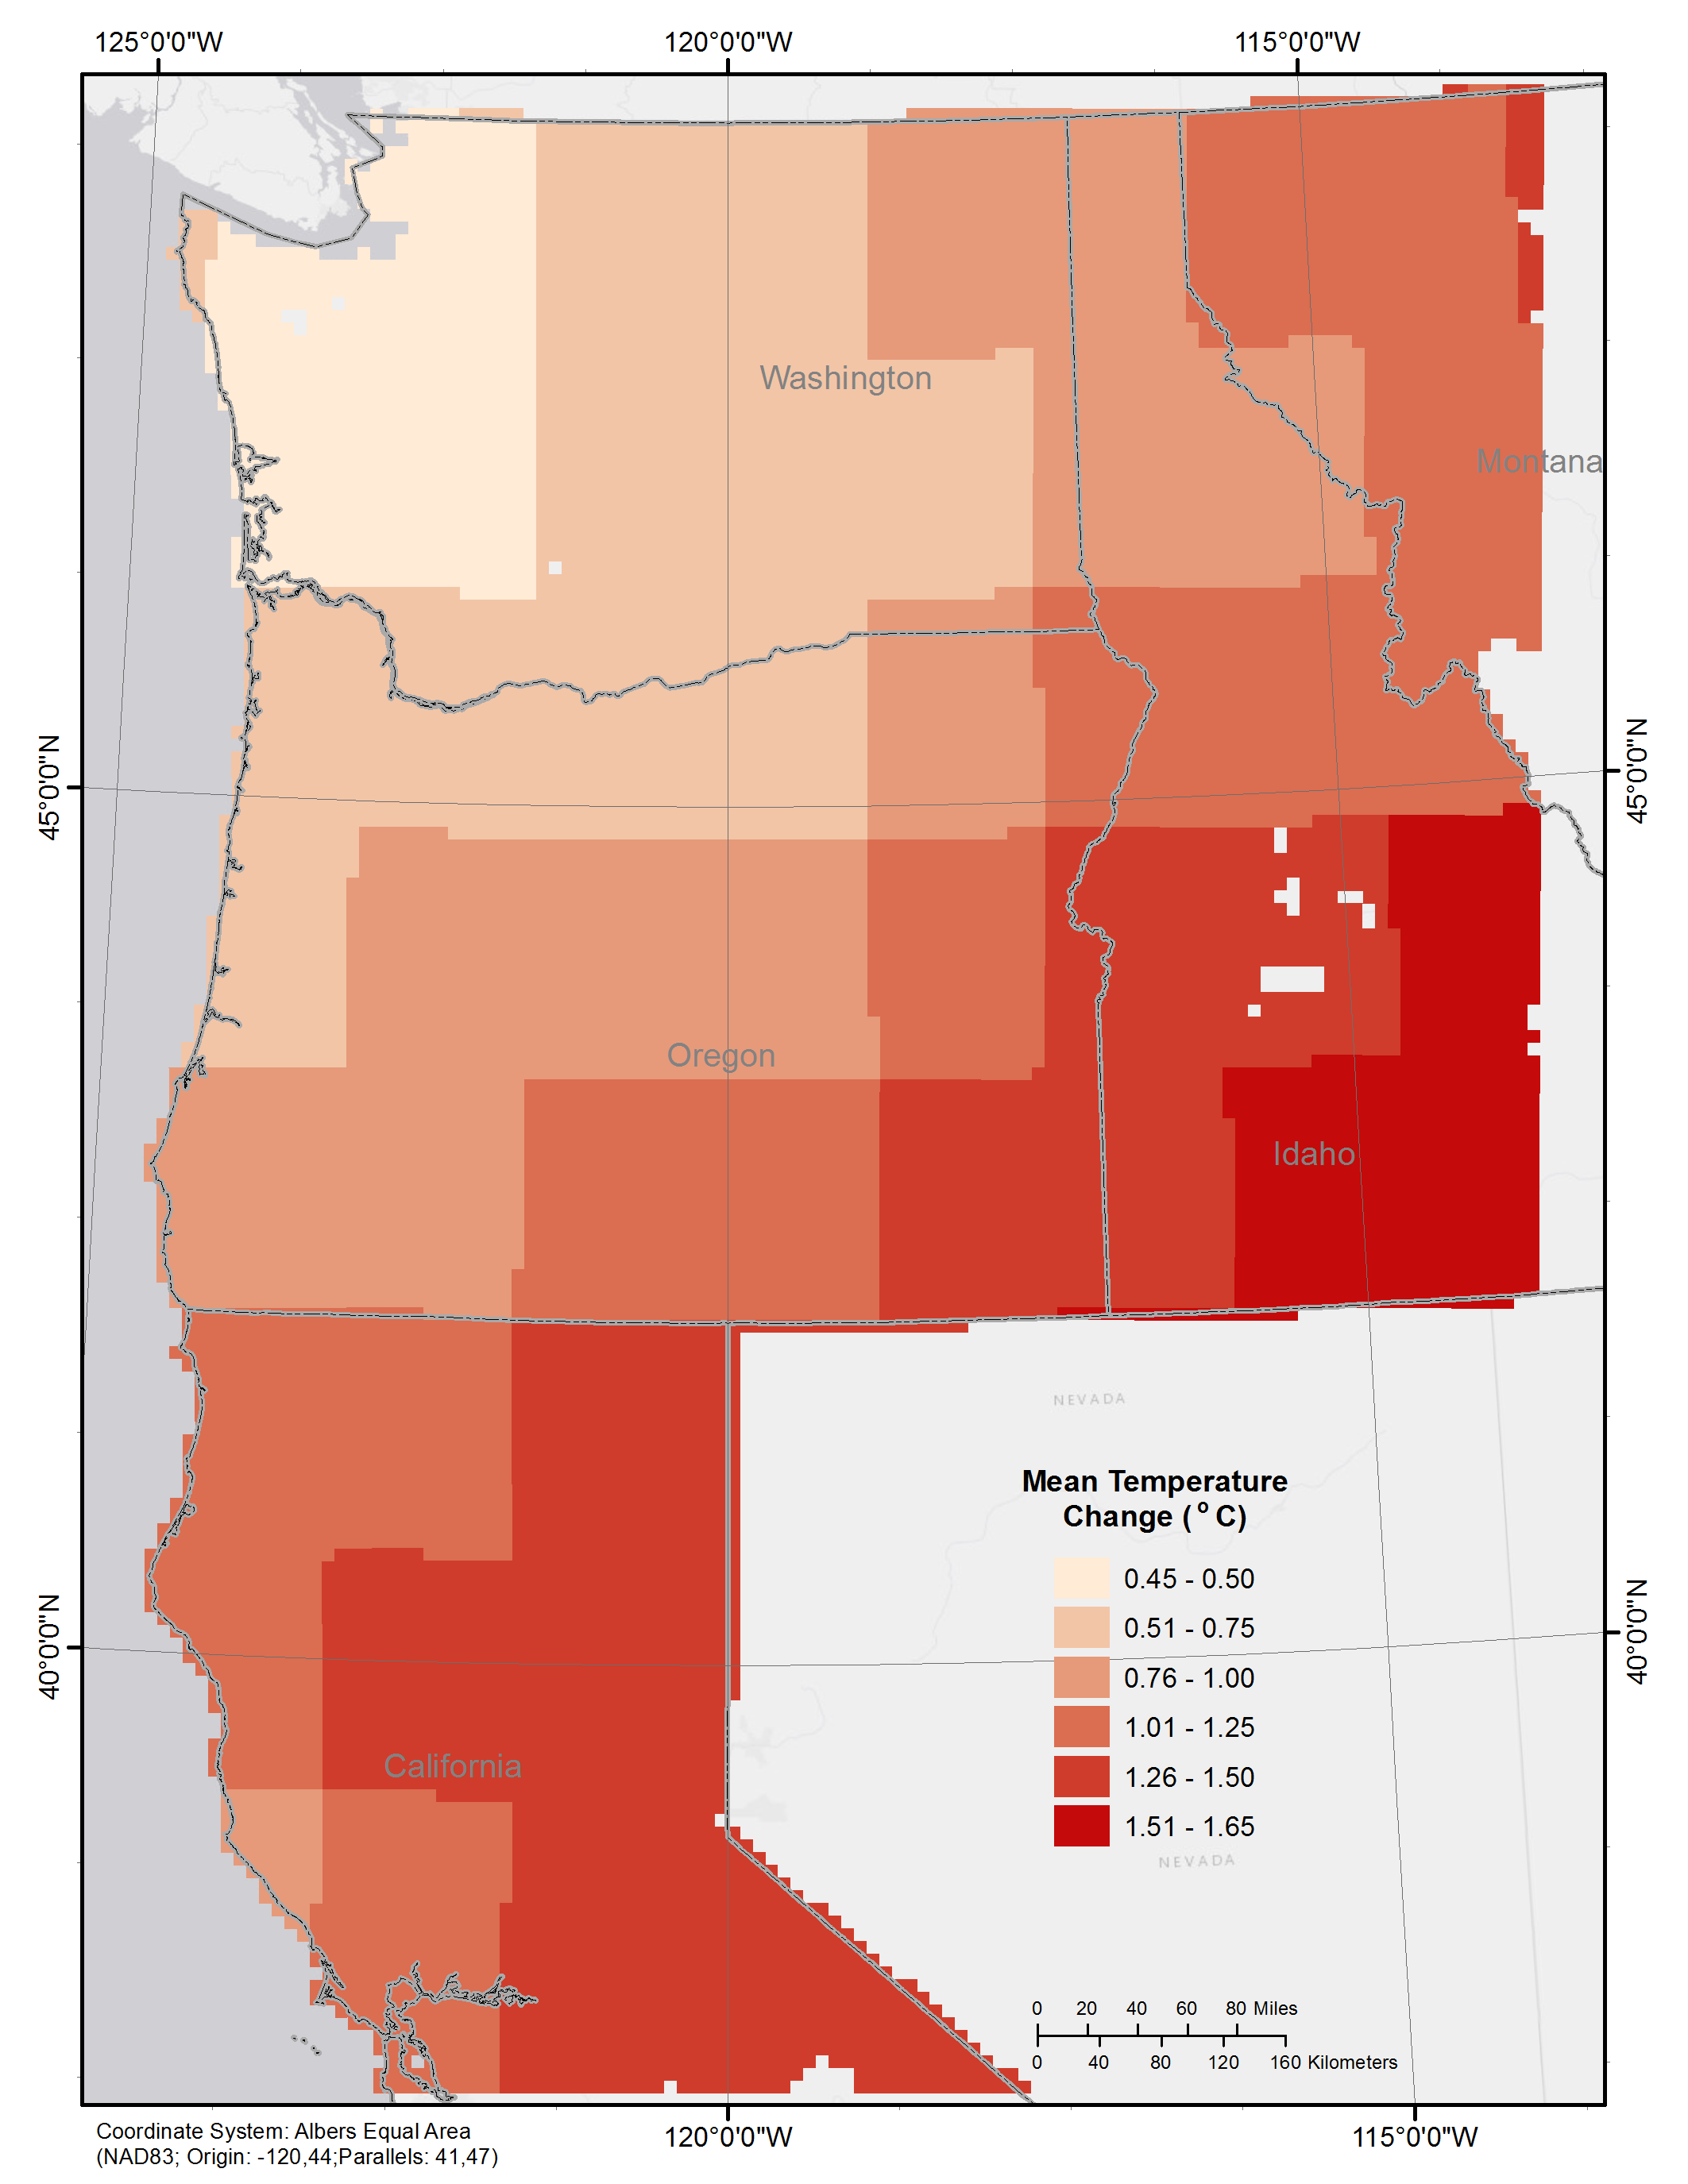
\includegraphics[width=0.45\linewidth]{temp_change}
  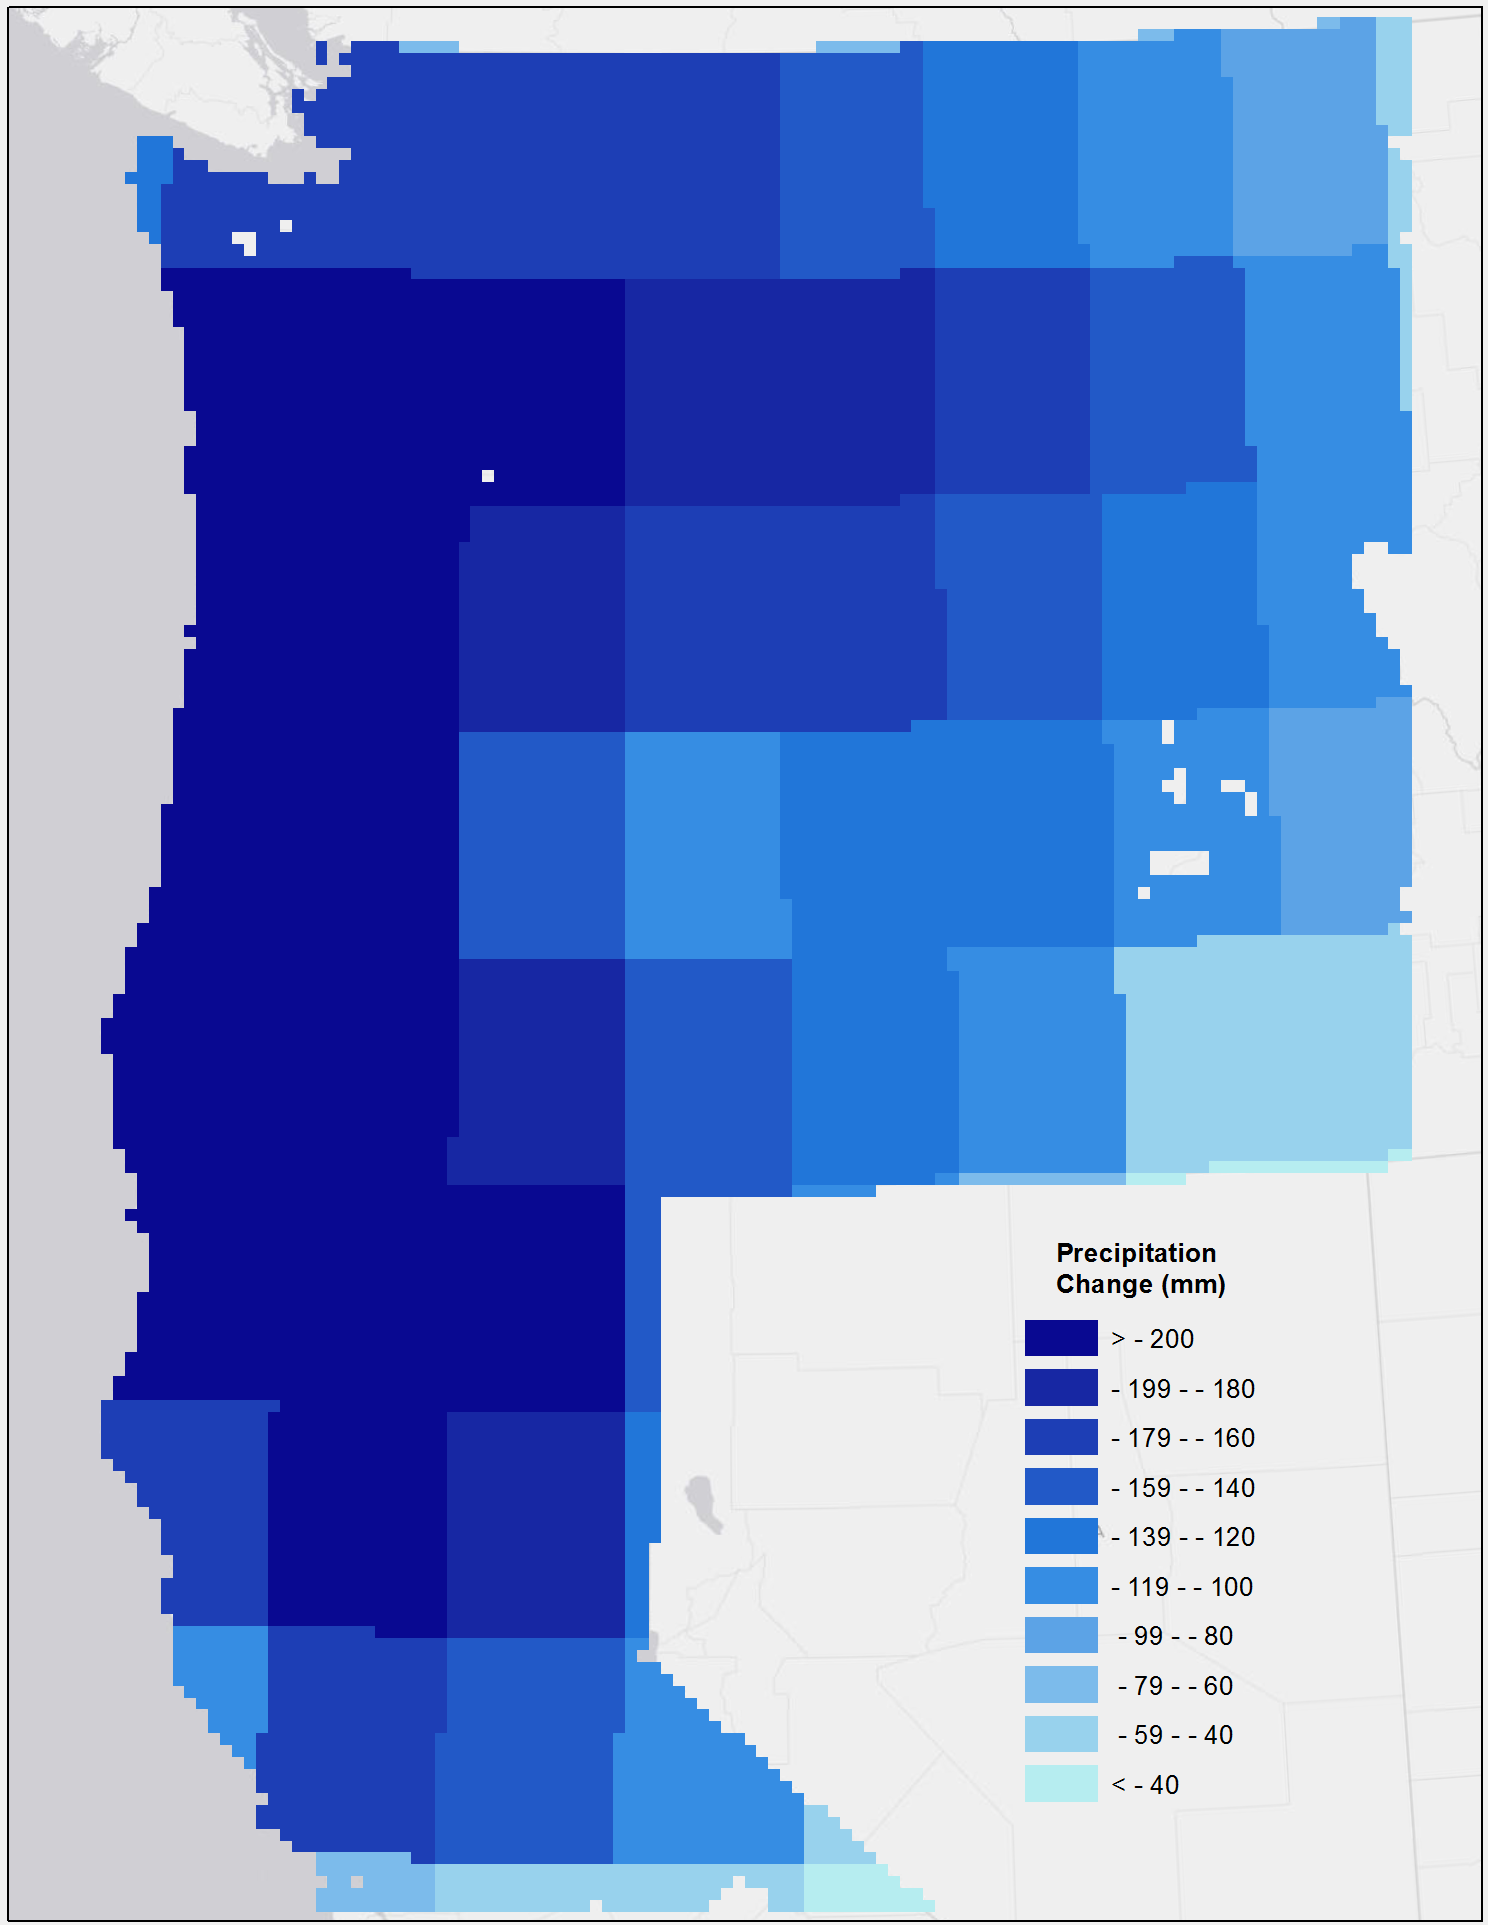
\includegraphics[width=0.45\linewidth]{precip_change.png}
  \caption{Predicted changes in temperature and precipitation under \ac{CCSM3} scenario A1B for plantation planted in 2040.}
  \label{fig:change}
\end{figure}

\section{Results and Discussion}

Seven representative poplar parameterizations were run over the
\ac{AHB} region, using both a model that included irrigation and one
that was nonirrigated.  The results were averaged over the set of
species parameters.  The runs were over an 18 total lifetime, with a
2.5 year initial coppicing event followed by 5 additional events on a
three year cycle.  Initial planting was in March, with all coppicing
events occurring in November.  The 6 total harvest events were
annualized over the 18 year time span to report predicted yields on a
per year basis.

Finally, the layer of current croplands was used to mask the yield
maps to include only those areas where irrigation is likely, to
determine an overall predicted irrigated yield.  The results show an
average yield over the entire region of 19.7 (Mg/ha).  3.8 (Mha) were
included in the estimate.  Yields were highest in the central valley
of California, a rich agricultural center, with similar yields along
the temperate western parts of Oregon and Washington.  Yields
decreased in the Northern plains, reaching lows in the Northeastern
section of the study region~(Figure~\ref{fig:irrigated_yield}).

\begin{figure}[hp]
  \centering
  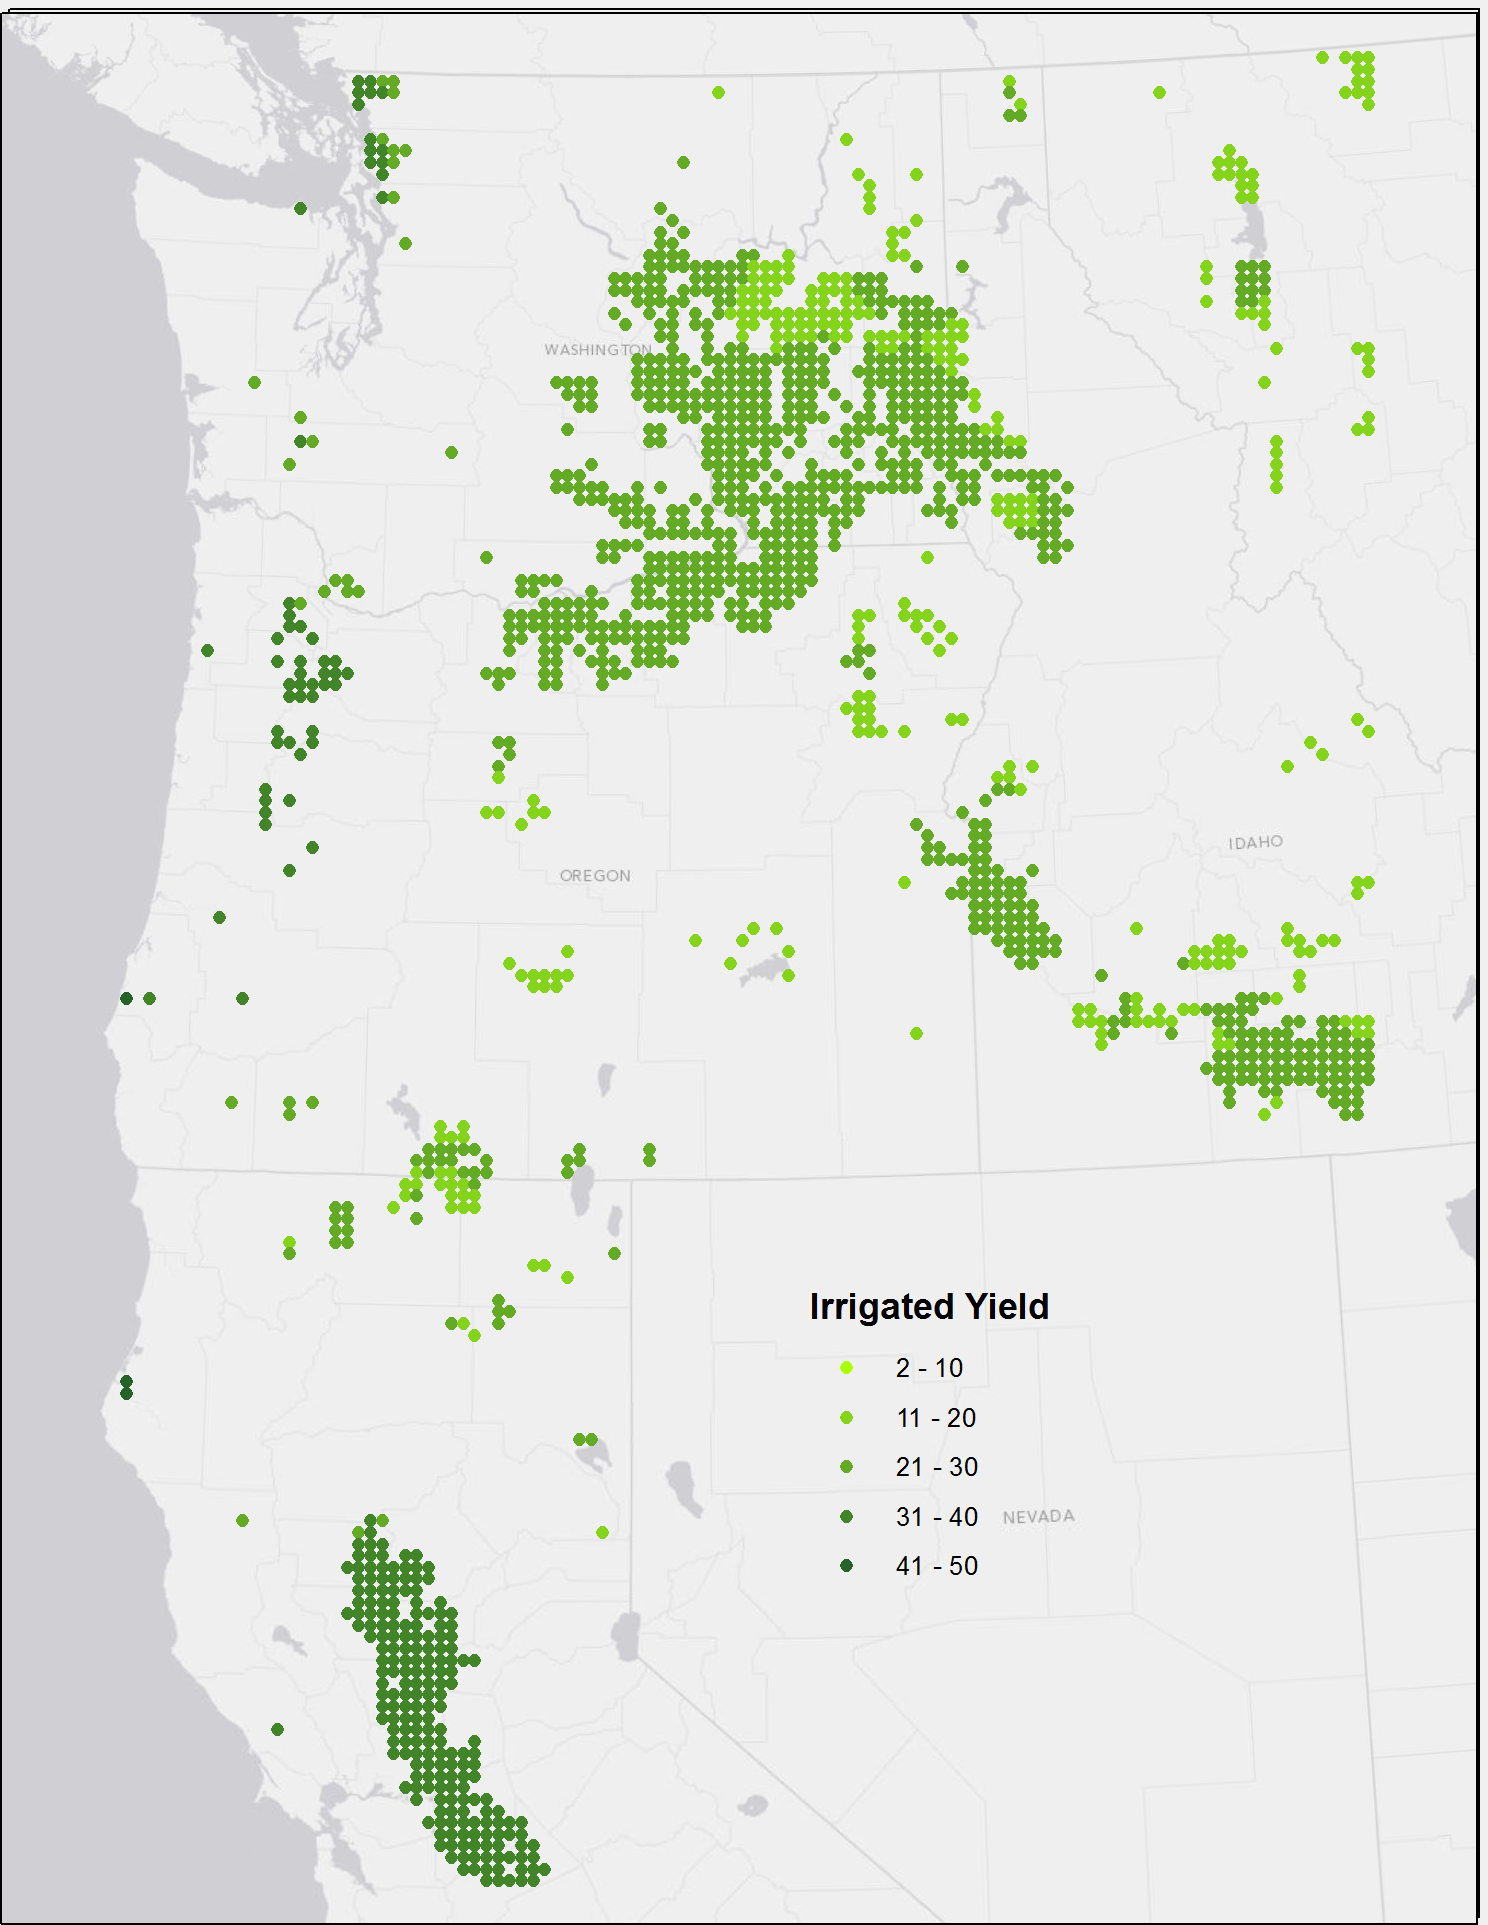
\includegraphics[width=1.0\linewidth]{irrigated_yield}
  \caption{Predicted annual irrigated yields for a 18 year 5 coppice plantation cycle for areas in the \ac{PNW} currently under agricultural practice.  The image only includes pixels with more that \%20 area identified as cropland.  The isolines on the maps describe the standard deviation over the 7 parameterizations.}
  \label{fig:irrigated_yield}
\end{figure}

Similarly, the nonirrigated yield predictions were masked with the
areas excluded in the land suitability study to include those areas
likely to support nonirrigated poplar plantations.  Results for the
nonirrigated lands predict a yield of 6.6 (Mg/ha) over an area under
consideration of 5.7 (Mha).  In the case of nonirrigated yields, the
highest yields were along the Pacific coast where precipitation is
most plentiful, and more uniform in the inland areas of the \ac{AHB}
region~(Figure~\ref{fig:nonirrigated_yield}).

\begin{figure}[hp]
  \centering
  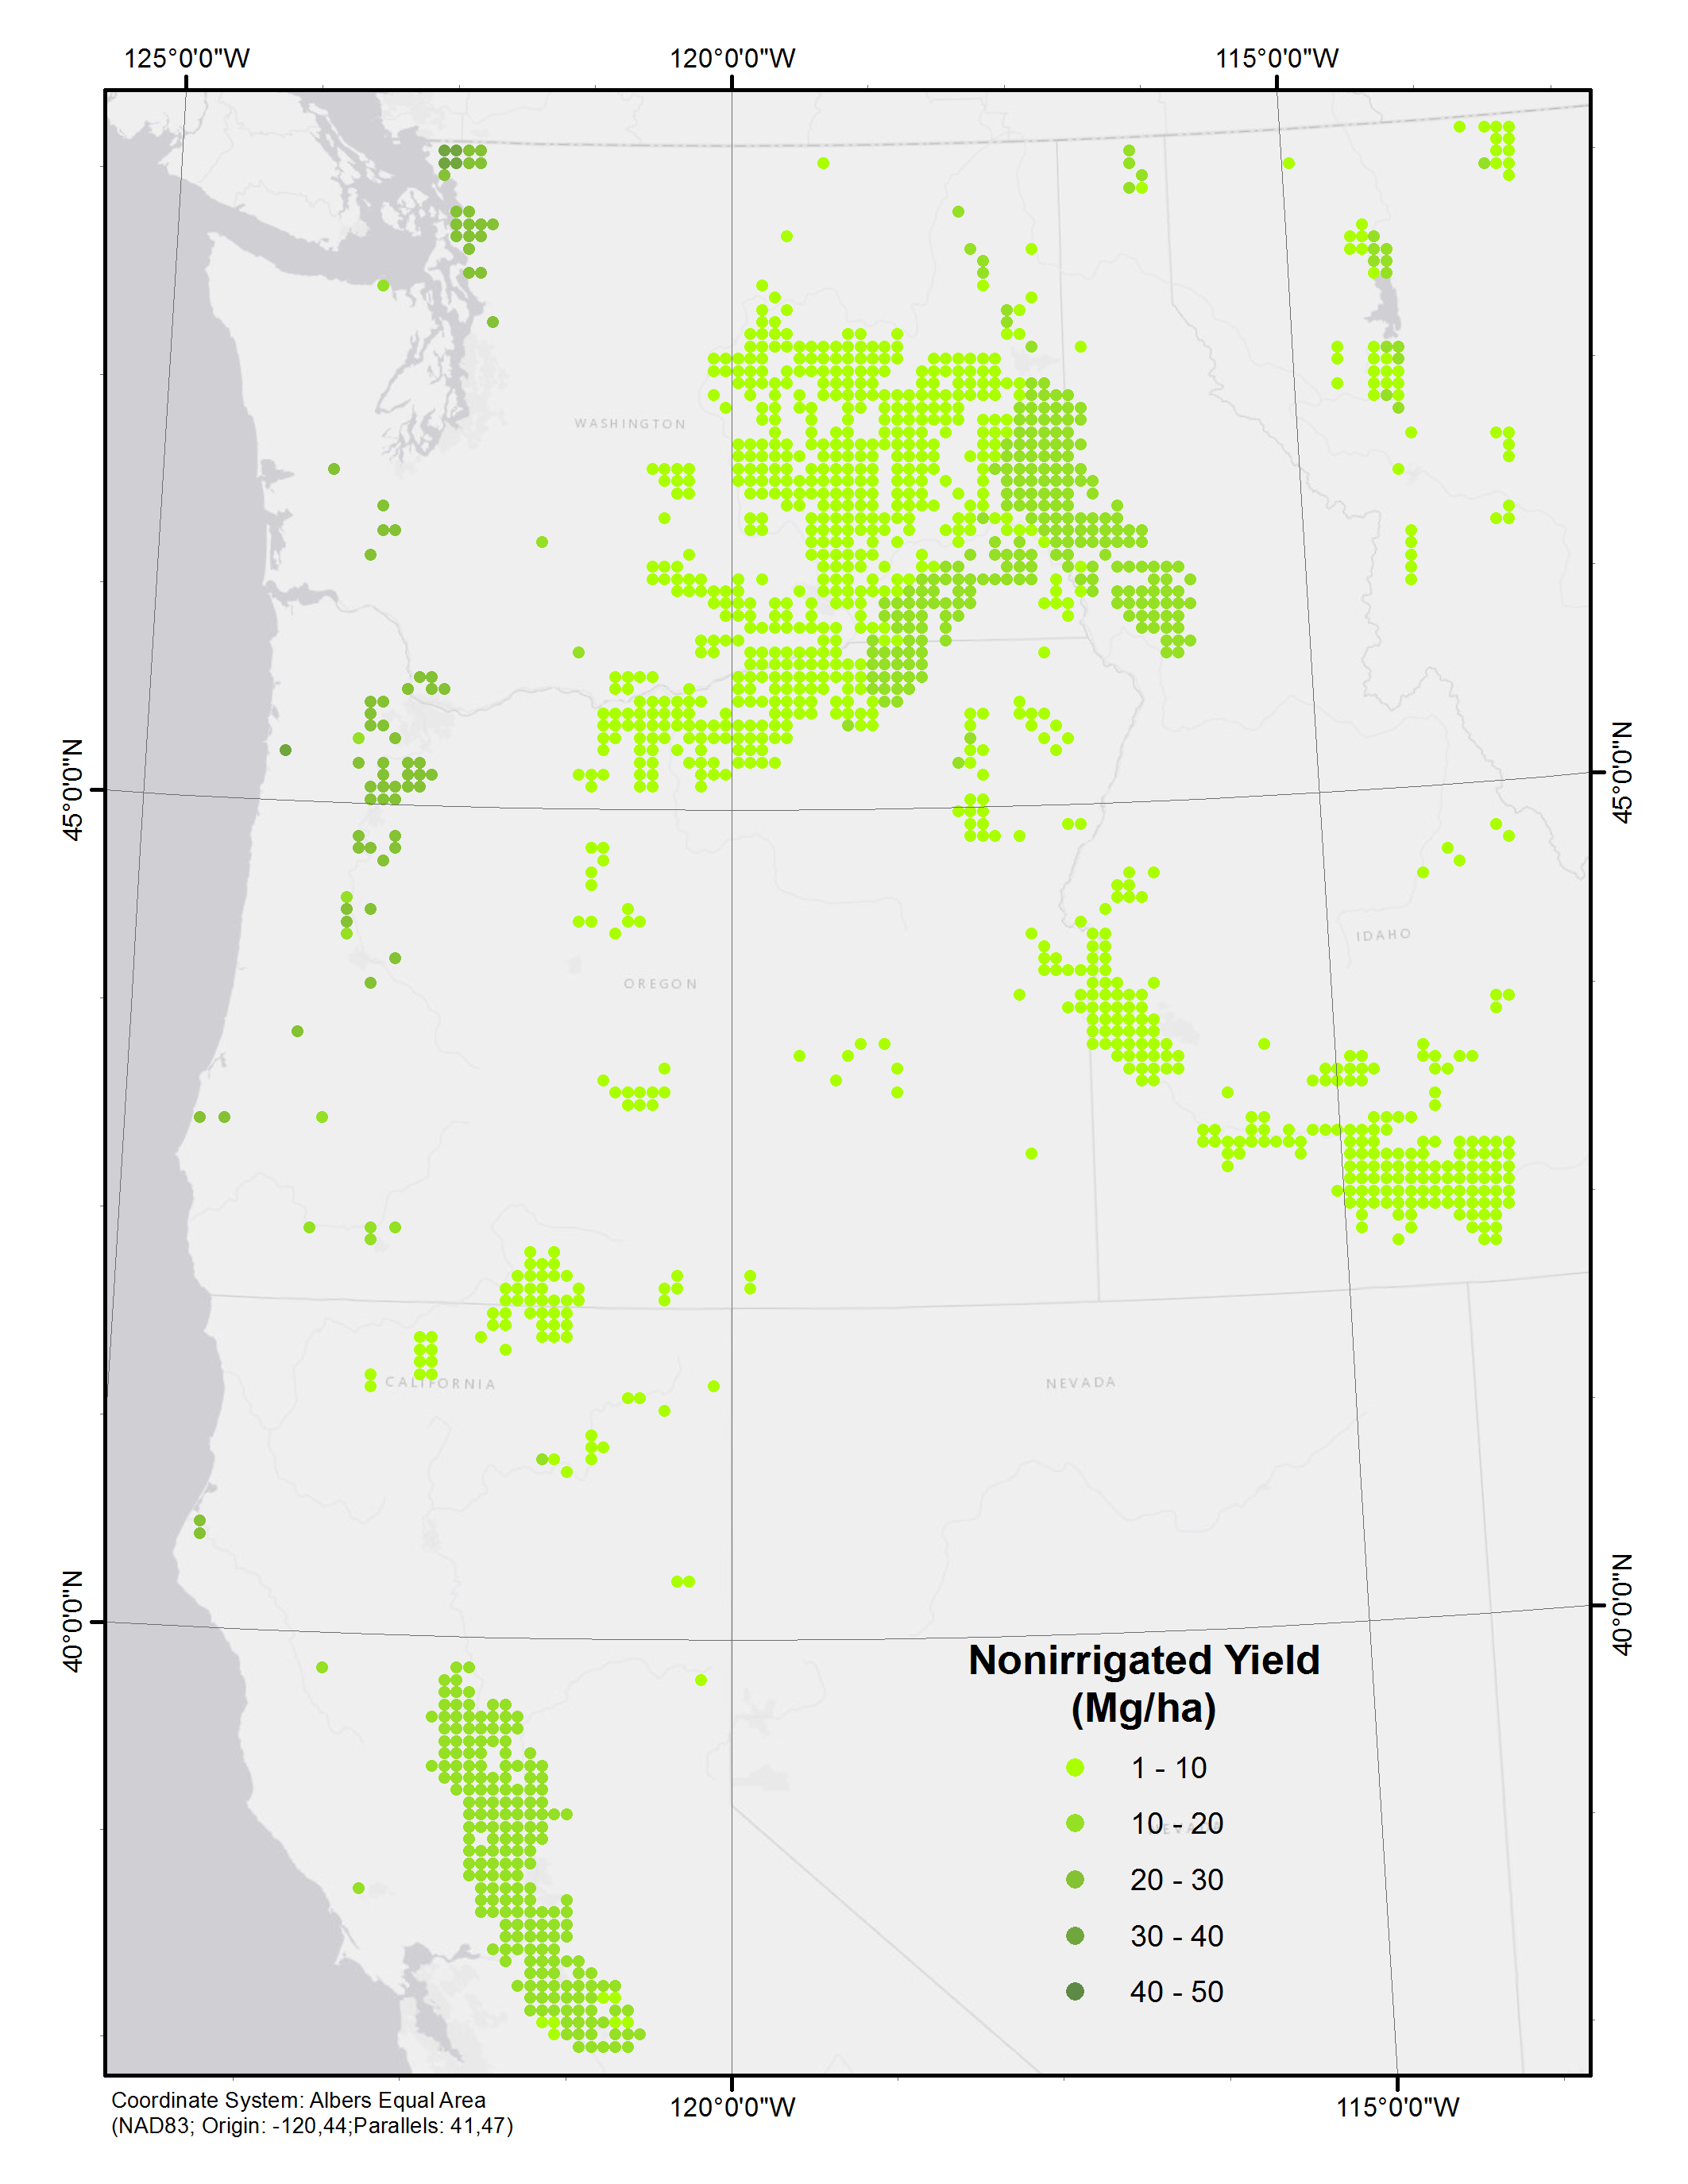
\includegraphics[width=1.0\linewidth]{nonirrigated_yield}
  \caption{Predicted annual nonirrigated yields for a 18 year 5 coppice plantation cycle for areas in the \ac{PNW} identified as rangeland or marginal land.  The image only includes pixels with more than \%20 area identified as marginal or rangeland.  The isolines on the maps describe the standard deviation over the 7 parameterizations.}
  \label{fig:nonirrigated_yield}
\end{figure}

%\subsection{Climate Change}
%\label{sec:climate-change}

To assess the predicted change in yields from the A1B example study,
the model was rerun with the same parameters as the previously, but
with the predicted changes in temperature and precipitation.  The
results were averaged and summarized as above to determine annualized
yields.  The yields were then compared to the current yield estimates
to determine the difference in predicted yields under that one example
climate change scenario.  

Under irrigated conditions, the higher predicted temperatures
generally improve yields through most of the region, with the
exception of California, where high temperatures often limit monthly
growth.  Changes in yield are modest in the areas with the highest
yields and more significant in the colder Northern and central
regions~(Figure~\ref{fig:irrigated_yield}).
 
\begin{figure}[hp]
  \centering
  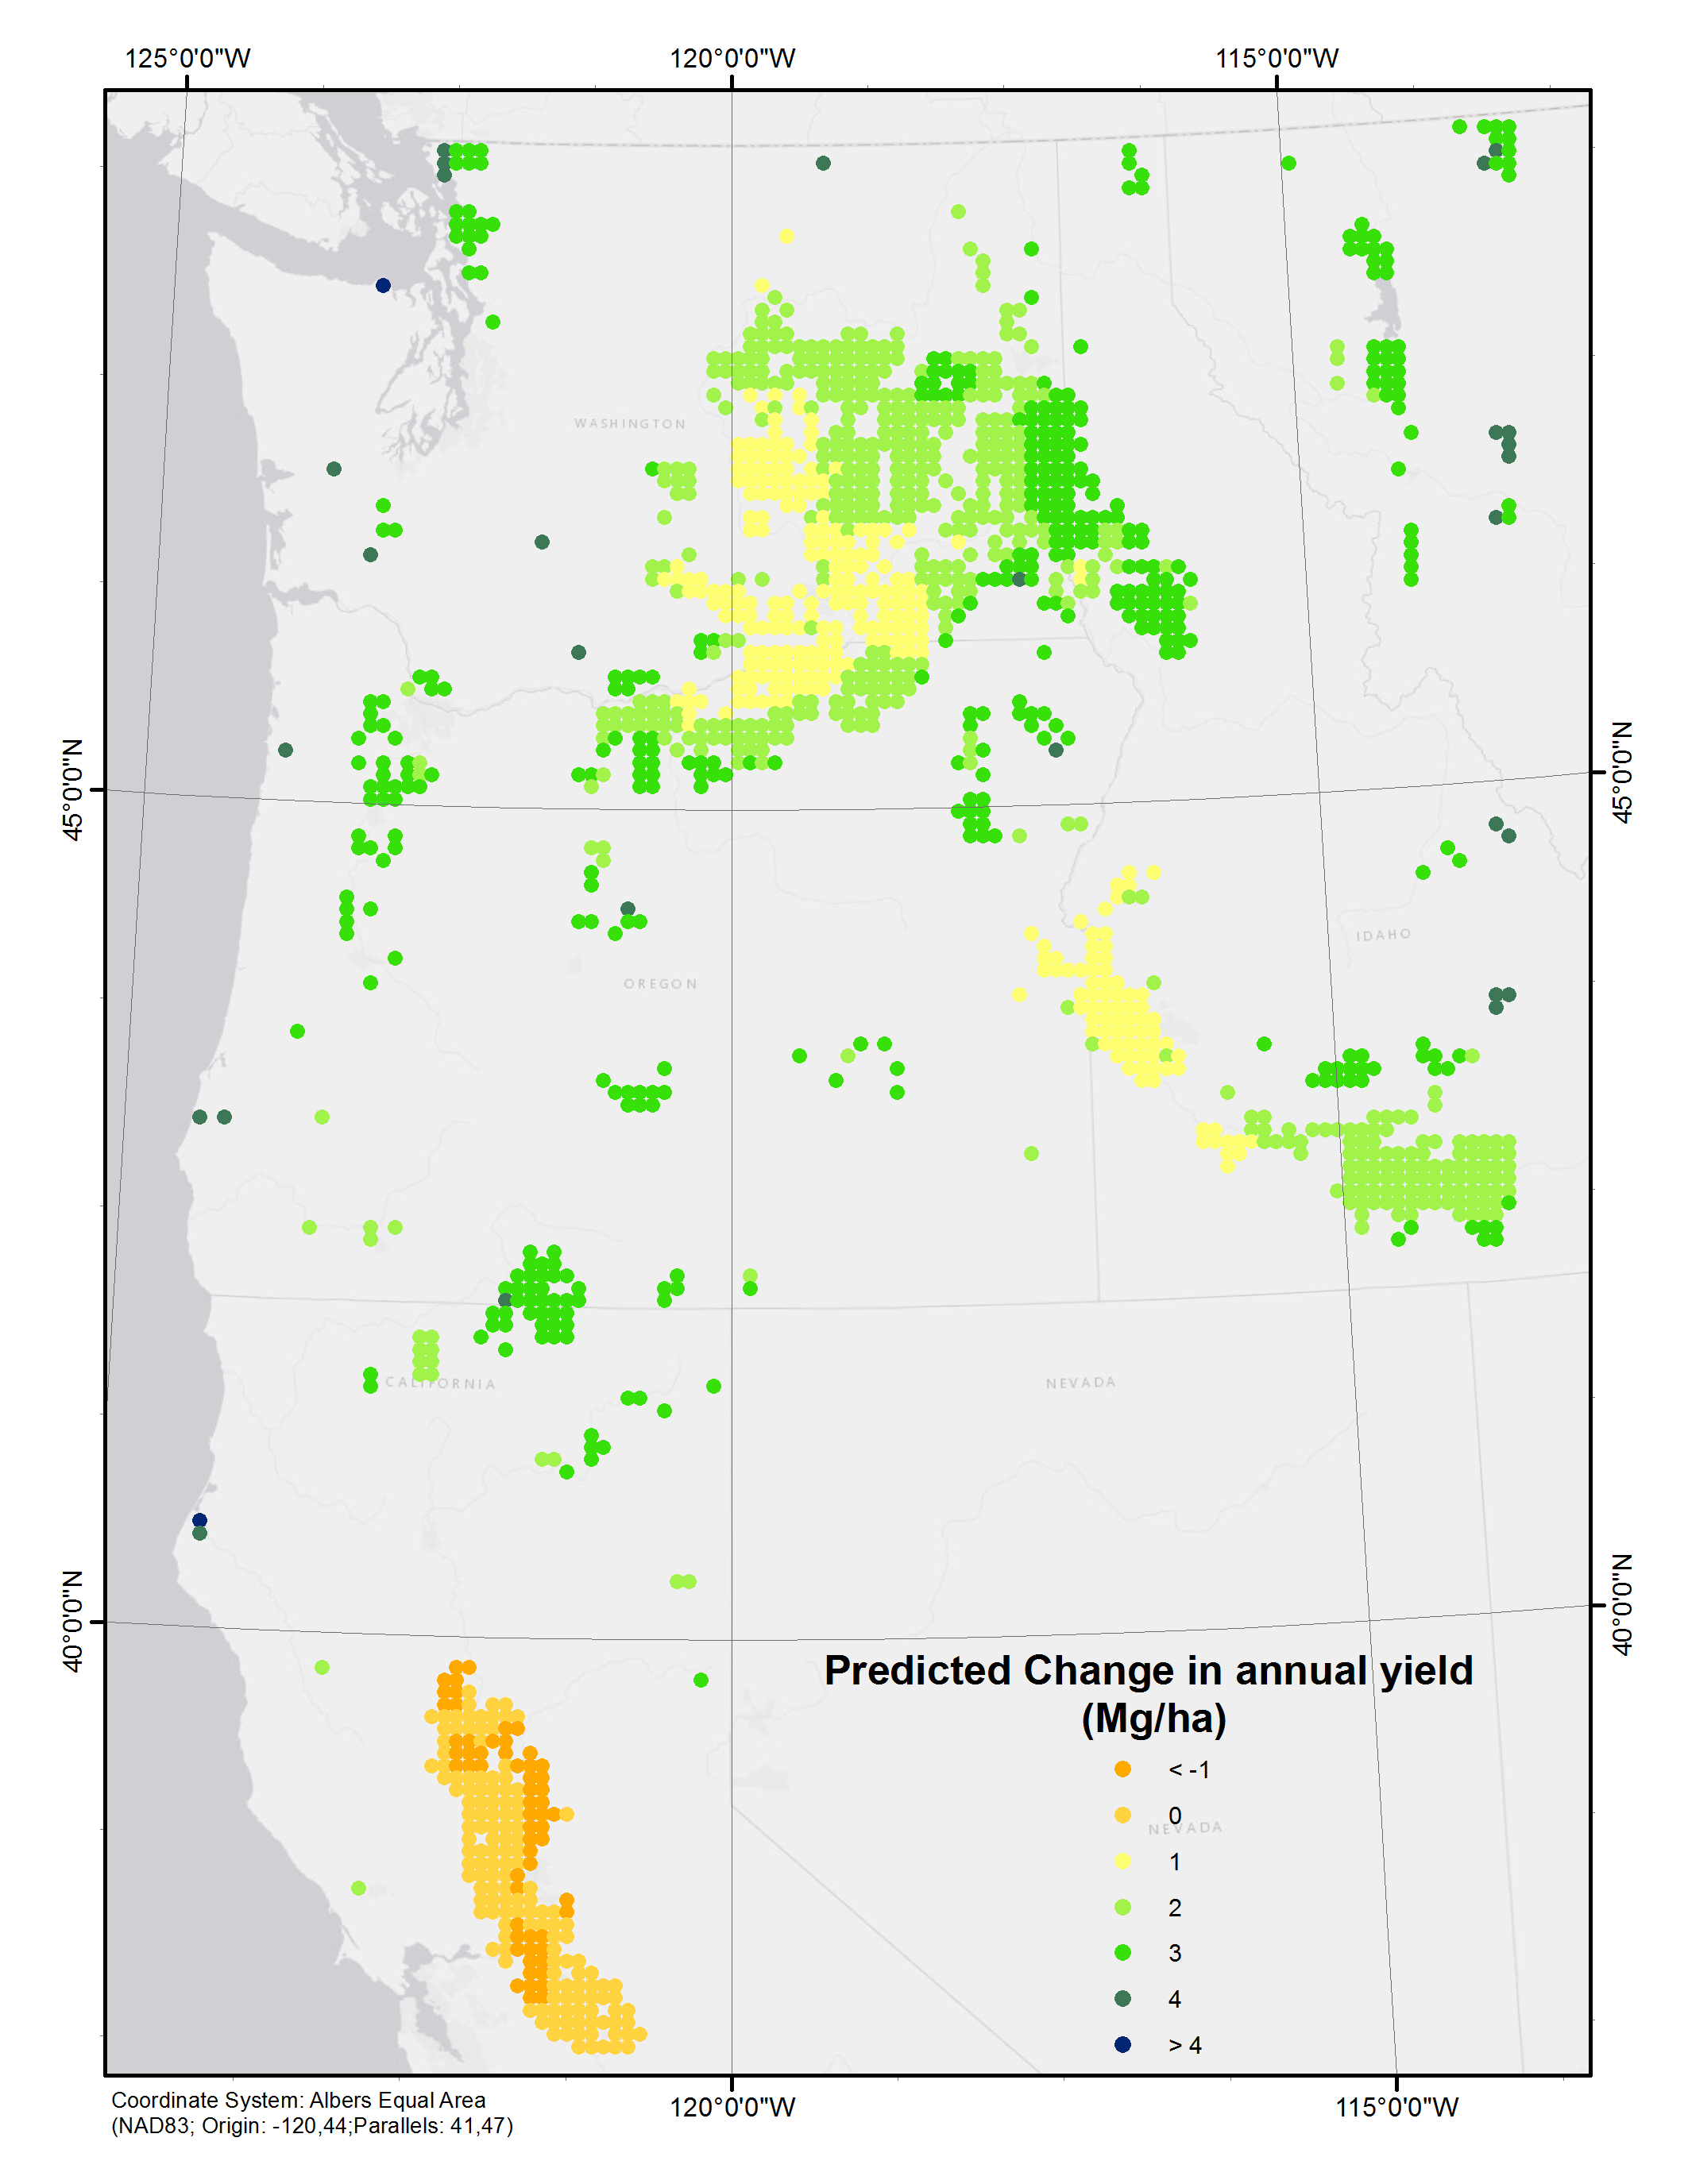
\includegraphics[width=1\linewidth]{climate_irrigated}
  \caption{Changes in predicted irrigated yield for \ac{CCSM3} scenario A1B
    for a plantation planting in 2040-2058.}
  \label{fig:new_irrigated}
\end{figure}

For nonirrigated plantations, the predicted decrease in precipitation
decreases yields along the areas with the current highest yields,
along the wet Pacific coast.  Higher temperatures continue to increase
yields in most of the inland areas~(Figure~\ref{fig:new_nonirrigated})

\begin{figure}[hp]
  \centering
  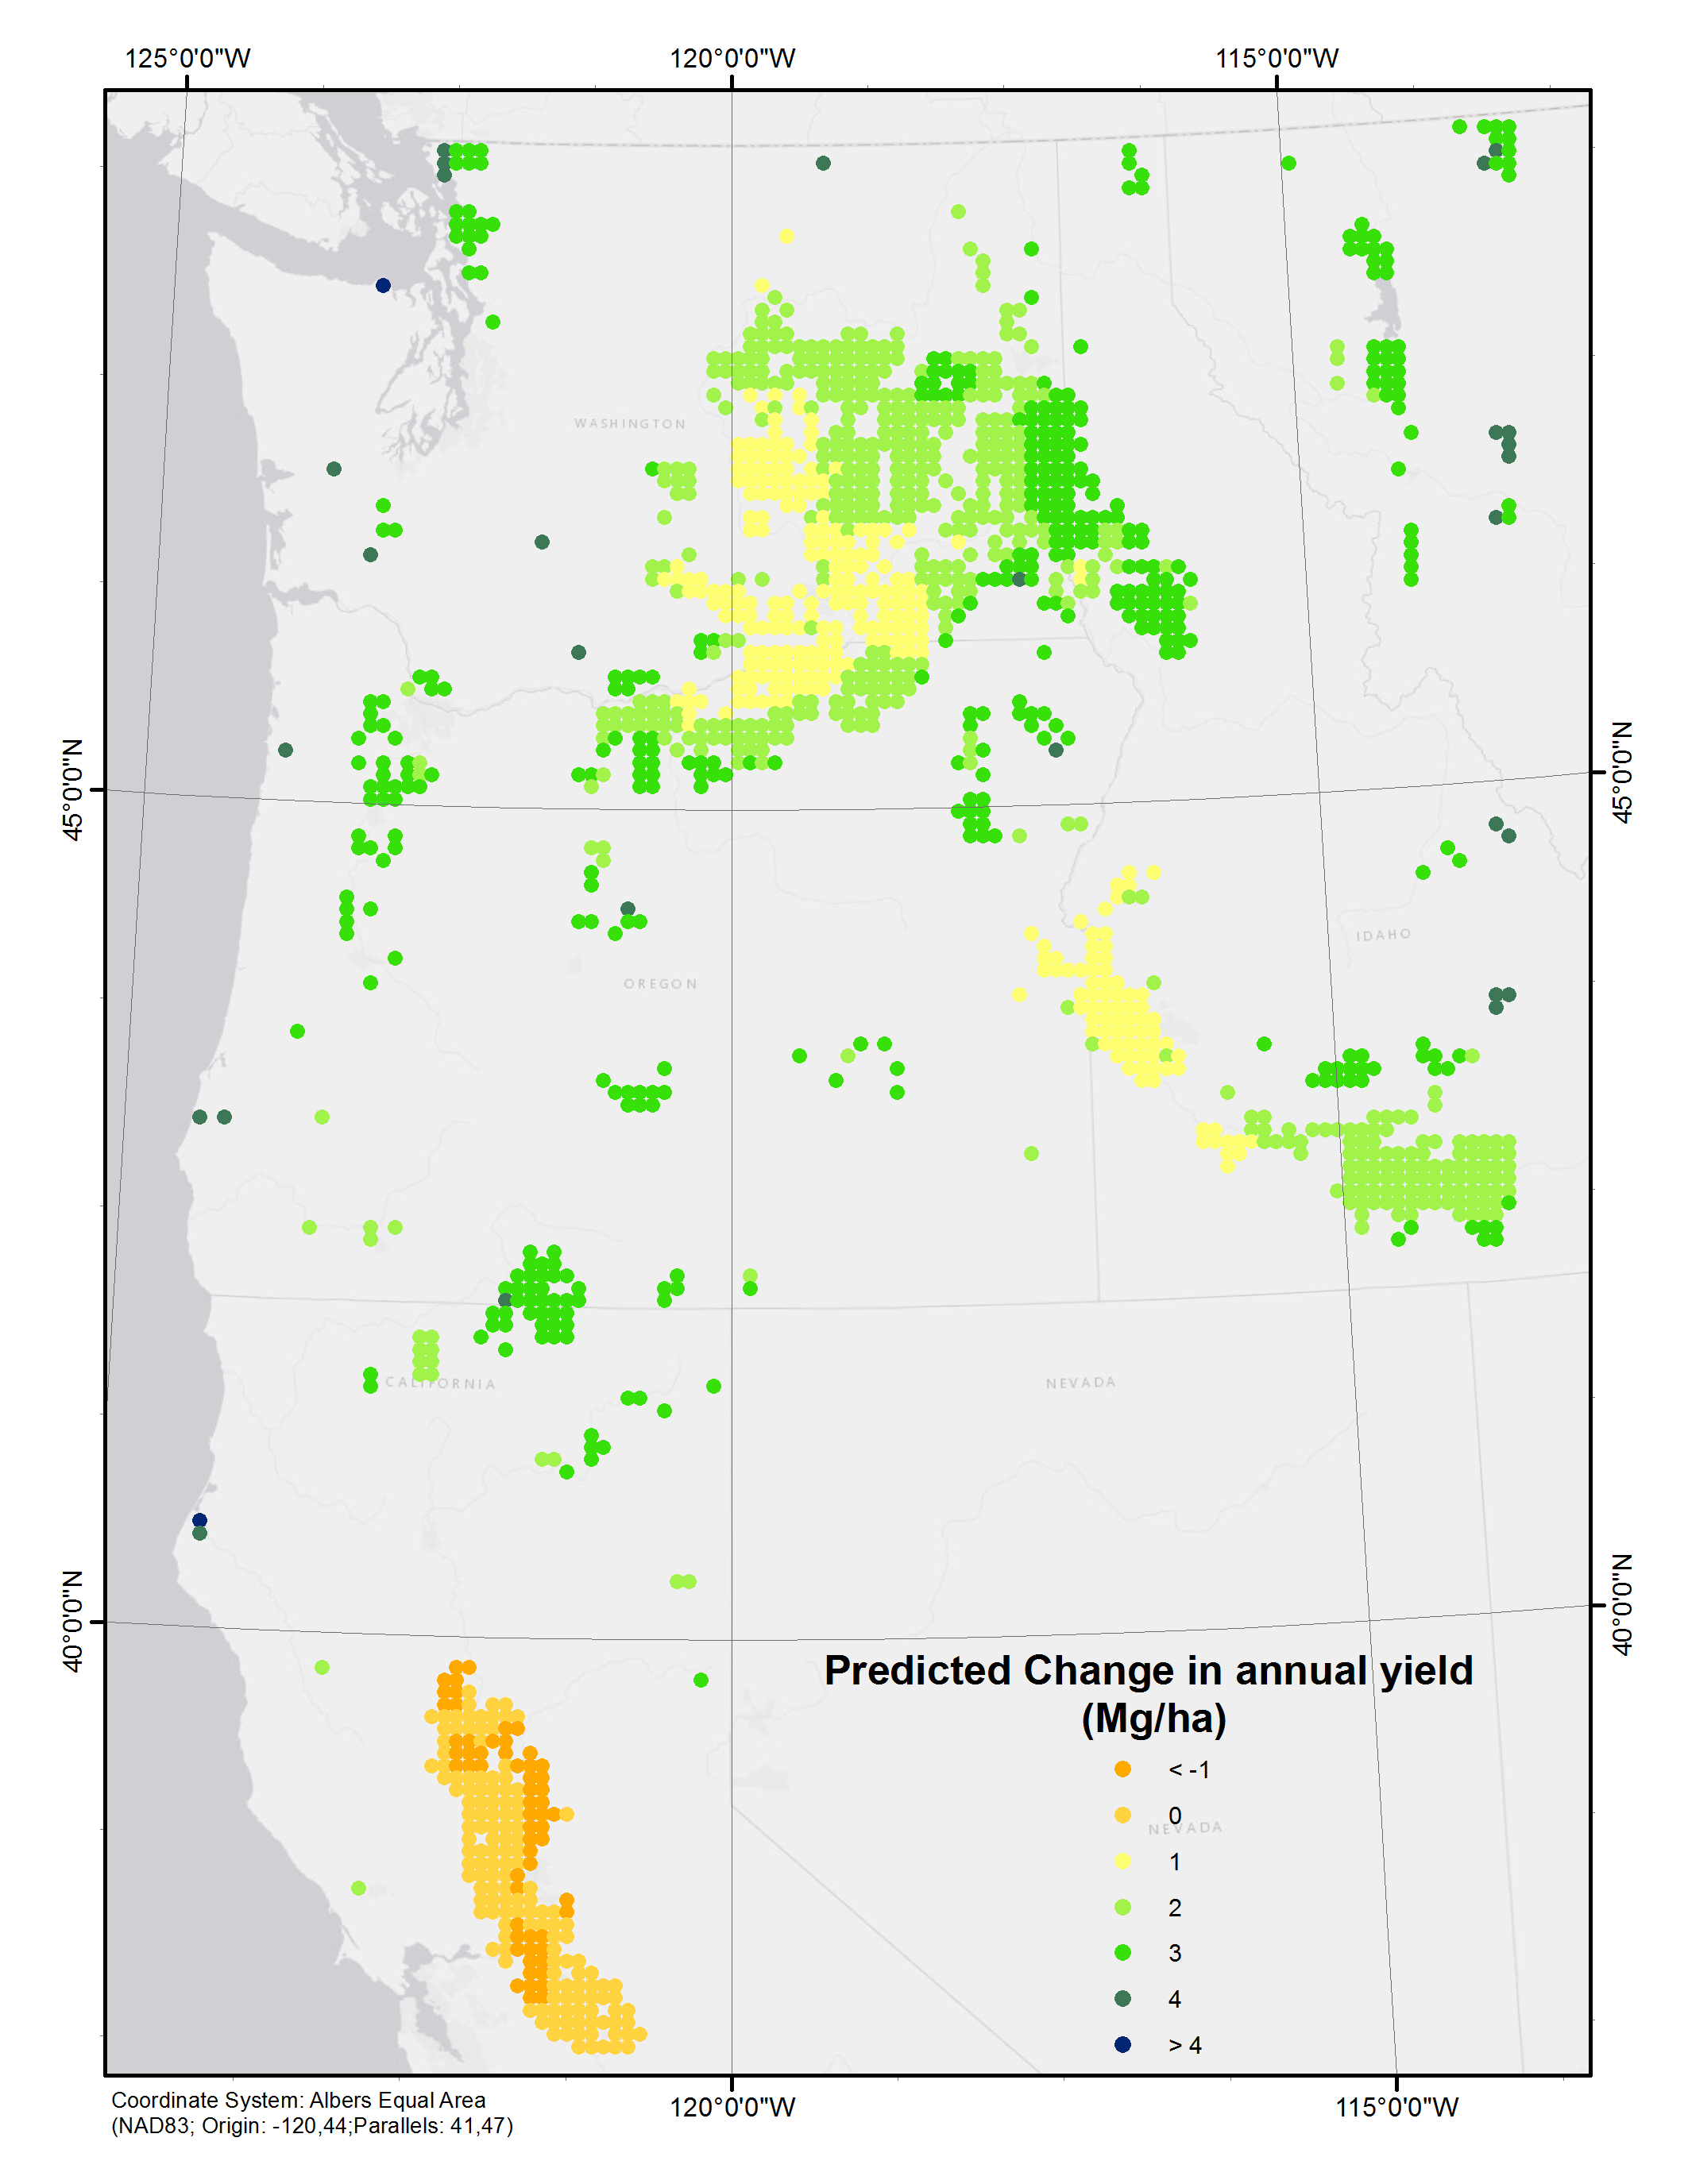
\includegraphics[width=1\linewidth]{climate_irrigated}
  \caption{Changes in predicted nonirrigated yield for \ac{IPCC} scenario A1B
    for a plantation planting in 2040-2058.}
  \label{fig:new_nonirrigated}
\end{figure}

These change estimations can inform both the individual farmer in terms of
predicting long term viability of poplar plantations as a \ac{SRWC}
feedstock, as well as regional estimations on the mid-term ability of
such a feedstock to provide an expected harvest, and therefore an
expected level of biofuel production.  Not only changes in expected
overall yields, but changes in the spatial distribution of the yields
can have impacts on economic analysis of a \ac{SRWC} based biofuel
industry in the \ac{PNW}.  

These example climate change yield change predictions are
illustrative, but the mean change in yields are not necessarily the
most robust estimation of changes in yield predictions.  First, the
\ac{CCSM3} models are not tuned to the relatively short time frame of
looking forward 25-50 years.  In addition, while temperature increases
are consistently predicted, the change in precipitation is less
uniformly predicted among different models and scenarios. 

With appropriate input information, the \ac{3pg} model can predict
yields for the entire \ac{PNW} study region, under various irrigation
scenarios.  When linked with models of crop adoption and biorefinery
models the economic viability of poplar as a biofuel feedstock can be
examined.
 
For example, in the \ac{AHB} project, a companion model, the
\acf{BCAM}, predicts price levels where poplar competes with existing
crops in about 35 different general cropping regions in the \ac{PNW}.
The spatially distributed yield predictions inform the \ac{BCAM}
model.  For irrigated land, current yields are input into a \ac{BCAM}
model where they compete with existing crops to determine their
economic viability.  The yield predictions also include predictions in
required water, and the \ac{BCAM} model manages water availability by
balancing any water needs from the poplar with water saved from crops
taken out of the agricultural system.  Outputs of the \ac{BCAM} model
show at what farm gate price (\$/Mg) poplar becomes an economically
viable product.
 
For non-irrigated land, marginal and under utilized lands can be added
into the overall agricultural economy as newly utilized lands.  For
nonirrigated plantations, crop budgets can give estimates of farm gate
costs (\$/Mg) which are affected by the predicted yields.

Both the irrigated and nonirrigated regions, total amount of available
feedstock for a particular farm gate price can then be estimated.
These are also spatially distributed.  Another \ac{AHB} model, the
\acf{GBSM} takes as inputs these spatially distributed price curves,
and use them in coordination with feedstock transport and refinery
costs, to optimize the size and location of a set of refineries, to
most efficiently process the poplar into a biofuel.  The results from
the \ac{GBSM} model include both the predicted refinery system as well
as an anticipated cost of fuel itself.  The current resolution of the
\ac{AHB} grid is designed to provide a workable input for the solver
of the \ac{GBSM} model.  Subsequent model runs at a finer scale can
test the best scales for application of these models.

\section{Conclusions}
\label{sec:conclude}

With the addition of the coppicing model, the \ac{3pg} model can be
used to predict poplar yields for the \ac{PNW} region.  The model can
include irrigation which increases yields from most areas in the region.  

With additional layers showing current croplands, areas the can be
irrigated are identified.  Poplar suitability maps limit consideration
on nonirrigated plantations to regions that are amenable to such
management.

Spatially distributed yield predictions inform regional models as to
the expected costs of producing a poplar biofuel feedstock and the
price at which that commodity becomes economically viable.

This work is supported by an Agriculture and Food Research Initiative
Competitive Grant no. 2011-68005-30407 from the USDA National
Institute of Food and Agriculture (NIFA).

%% The Appendices part is started with the command \appendix;
%% appendix sections are then done as normal sections
%% \appendix

%% \section{}
%% \label{}

%% If you have bibdatabase file and want bibtex to generate the
%% bibitems, please use
%%
\bibliographystyle{elsarticle-num} 
\bibliography{ahb-pnw}

%% else use the following coding to input the bibitems directly in the
%% TeX file.

% \begin{thebibliography}{00}

% %% \bibitem{label}
% %% Text of bibliographic item

% \bibitem{}

% \end{thebibliography}

\end{document}
\endinput
%%
%% End of file `elsarticle-template-num.tex'.

%  LocalWords:  dataset Albers landcover postgresql geospatial SQL
%  LocalWords:  postgis PLSQL Javascript timestep coppicing datasets
%  LocalWords:  biorefinery aboveground coppiced biofuels feedstock
%  LocalWords:  SRWC parameterized physiographic orographic Isolines
%  LocalWords:  isolines parameterizations
